\documentclass[aspectratio=1610,10pt]{beamer}

% \usepackage{algorithmic}
\usepackage[noalgohanging,lined,noend,linesnumbered,onelanguage,portuguese,portuguesekw]{algorithm2e}
\SetAlCapSkip{1.5ex}
% \SetAlFnt{\tiny }
% \SetAlFnt{\scriptsize }
\SetAlFnt{\small}
\setlength{\algomargin}{0em}
\SetInd{.3em}{.5em}
\usetheme[progressbar=frametitle]{metropolis}
\usepackage{appendixnumberbeamer}
\usepackage{booktabs}
\usepackage{xspace}
\usepackage[brazil]{babel}
\usepackage[utf8x]{inputenc}
\usepackage{lmodern}
\usepackage[alf]{abntex2cite}
% \usepackage{ragged2e}
\usepackage{graphicx}
\usepackage{caption}
\usepackage{subcaption}

\newcommand{\printorientador}{<Orientador>}
\newcommand{\orientador}[1]{\renewcommand{\printorientador}{#1}}
\newcommand{\printagradecimento}{<agradecimento>}
\newcommand{\agradecimento}[1]{\renewcommand{\printagradecimento}{#1}}

\setbeamertemplate{title page}{
    \begin{minipage}[c][\paperheight]{\textwidth}
        \ifx\inserttitlegraphic\@empty\else\usebeamertemplate*{title graphic}\fi
        \vfill%
        \ifx\inserttitle\@empty\else\usebeamertemplate*{title}\fi
        \ifx\insertsubtitle\@empty\else\usebeamertemplate*{subtitle}\fi
        \usebeamertemplate*{title separator}
        \begin{minipage}[t]{.5\textwidth}
            \ifx\beamer@shortauthor\@empty\else\usebeamertemplate*{author}\fi
            \ifx\insertdate\@empty\else\usebeamertemplate*{date}\fi
            \ifx\insertinstitute\@empty\else\usebeamertemplate*{institute}\fi
        \end{minipage}
        \begin{minipage}[t]{.5\textwidth}
            \vspace*{2em}
            \ifx\printorientador\@empty\else{
              \hspace{3.2em}\small Orientador: \textit{\printorientador} \par
            }\fi
        \end{minipage}%
        \vspace*{4em}
        \ifx\printagradecimento\@empty\else{
          \footnotesize\printagradecimento
        }\fi
        \vfill
        \vspace*{1mm}
    \end{minipage}
}

\newcommand{\fonte}[1]{\vspace{-1em}{\footnotesize\textbf{Fonte:} #1}}

\title[]{Uma Implementação Distribuída em Névoa do Algoritmo de Detecção de
Novidade em Fluxos de Dados MINAS}
% \subtitle{Seminários de Metodologia Científica}
\author{Luís Henrique Puhl de Souza}
\orientador{Prof. Dr. Hermes Senger}
\institute{
Universidade Federal de São Carlos \\
Centro de Ciências Exatas e de Tecnologia \\
Departamento de Computação \\
Programa de Pós-Graduação em Ciência da Computação}
% \date{\today}
\date{05 Julho 2021}
% \titlegraphic{\hfill\includegraphics[height=1.5cm]{logo.pdf}}
\agradecimento{Obrigado CNPq pelo suporte financiero (contrato 167345/2018-4).}

\newcommand{\minas}{MINAS\xspace}

\begin{document}

\maketitle

\begin{frame}[noframenumbering]{Índice}
  \setbeamertemplate{section in toc}[sections numbered]
  \tableofcontents[hideallsubsections]
\end{frame}

\section{Introdução}

\begin{frame}[fragile]{Introdução}
  \begin{itemize}%[<+- | alert@+>]
  % Contexto Geral
  \item Crescimento do número de dispositivos IoT e riscos associados;
  \begin{itemize}
    \item[$-$] Heterogeneidade de dispositivos;
    \item[$-$] Falta de atualizações de \emph{software};
    \item[$-$] Exemplo: \emph{Botnet} mirai, infectando cameras e roteadores, gerou
    $620 \ \mathrm{Gb/s}$ \cite{Kambourakis2017}.
  \end{itemize}
  % Contexto Específico
  \item Detecção de intrusão em redes:
  \begin{itemize}
    \item detecção por assinatura \emph{versus} anomalia;
    \item ambiente de névoa e redes IoT.
  \end{itemize}

  % Proposta
  \item Um sistema para detecção de intrusão em Redes IoT implementando em névoa;

  % hipótese
  \item A hipótese do trabalho é que o algoritmo MINAS pode ser distribuído em
  névoa reduzindo a latência sem redução na qualidade de classificação.

  \end{itemize}
  % \nota{pode falar:\\
  % - dificuldade de atualização de SW\\
  % - como foi o ataque MIRAI? (só curiosidade)\\
  % - capacidade de autodefesa? mesmo outros computadores não têm...}
\end{frame}


\section{Fundamentos}
\begin{frame}[fragile]{Fundamentos}
\begin{itemize}
  \item Fluxo de Dados e Métodos Detecção de Novidade;
  \item Plataformas de processamento distribuído de fluxos;
  \item Ambientes de computação Distribuída.
\end{itemize}
% \nota{Por que "seria dificil processar de forma centralizado"? [tg] corrigir no discurso}
\end{frame}

\begin{frame}[fragile]{Fundamentos}
  \metroset{block=fill}
  \begin{block}{Definição de Fluxo de Dados}
    
    \vspace{1mm}

    Um fluxo de dados (\textit{Data Stream}) é uma sequência massiva possivelmente
    ilimitada de exemplos multi-dimensionais $x_1, x_2, \dots, x_n, \dots$
    recebidos em instantes associados $t_1, t_2, \dots, t_n, \dots$
    \cite{Aggarwal2003}.
  \end{block}

  \metroset{block=transparent}
  \begin{alertblock}{Métodos Detecção de Novidade}
    
    \vspace{1mm}
    Métodos Detecção de Novidade (\emph{Novelty Detection}) lidam com o reconhecimento e
    classificação de exemplos em padrões que diferem de padrões anteriores
    \cite{Gama2010}.
    \begin{itemize}%[<+- | alert@+>]
      
      \item Evolução de Conceito (\emph{Concept Evolution}): surgimento de um conceito durante
      o fluxo;
      
      \item Mudança de Conceito (\emph{Concept Drift}, deriva ou desvio): modificação da
      distribuição de um padrão conhecido. A modificação pode ser repentina,
      incremental ou recorrente;
      
      \item Ruído e \emph{Outliers}: que não pertencem a um conceito ou
      pertencem a um conceito porém estão fora da distribuição conhecida.
      
    \end{itemize}
  \end{alertblock}
% \nota{Poderia explicar melhor a evolução de modelos, "concept drift"
% (precisa estudar um pouco + a teoria).}
\end{frame}

\begin{frame}[fragile]{Fundamentos - \minas}
  \begin{itemize}%[<+- | alert@+>]
    \item Modelo de aprendizado \emph{Offline-Online};
    \item Transformação dos dados analisados para o espaço $\mathbb{R}^d$;
    \item Modelo de classificação com \emph{Clusters};
    \item Função de classificação baseada em distância euclideana;
    \item Algoritmo de agrupamento para identificação de novos padrões;
    \item Classificação de novos padrões entre recorrência, extensão e novidade;
  \end{itemize}
% \nota{MINAS: Use figura!\\pseudocodigo?}
\end{frame}

\begin{frame}[fragile]{Fundamentos - \minas}
\begin{figure}[ht]
  \centering
  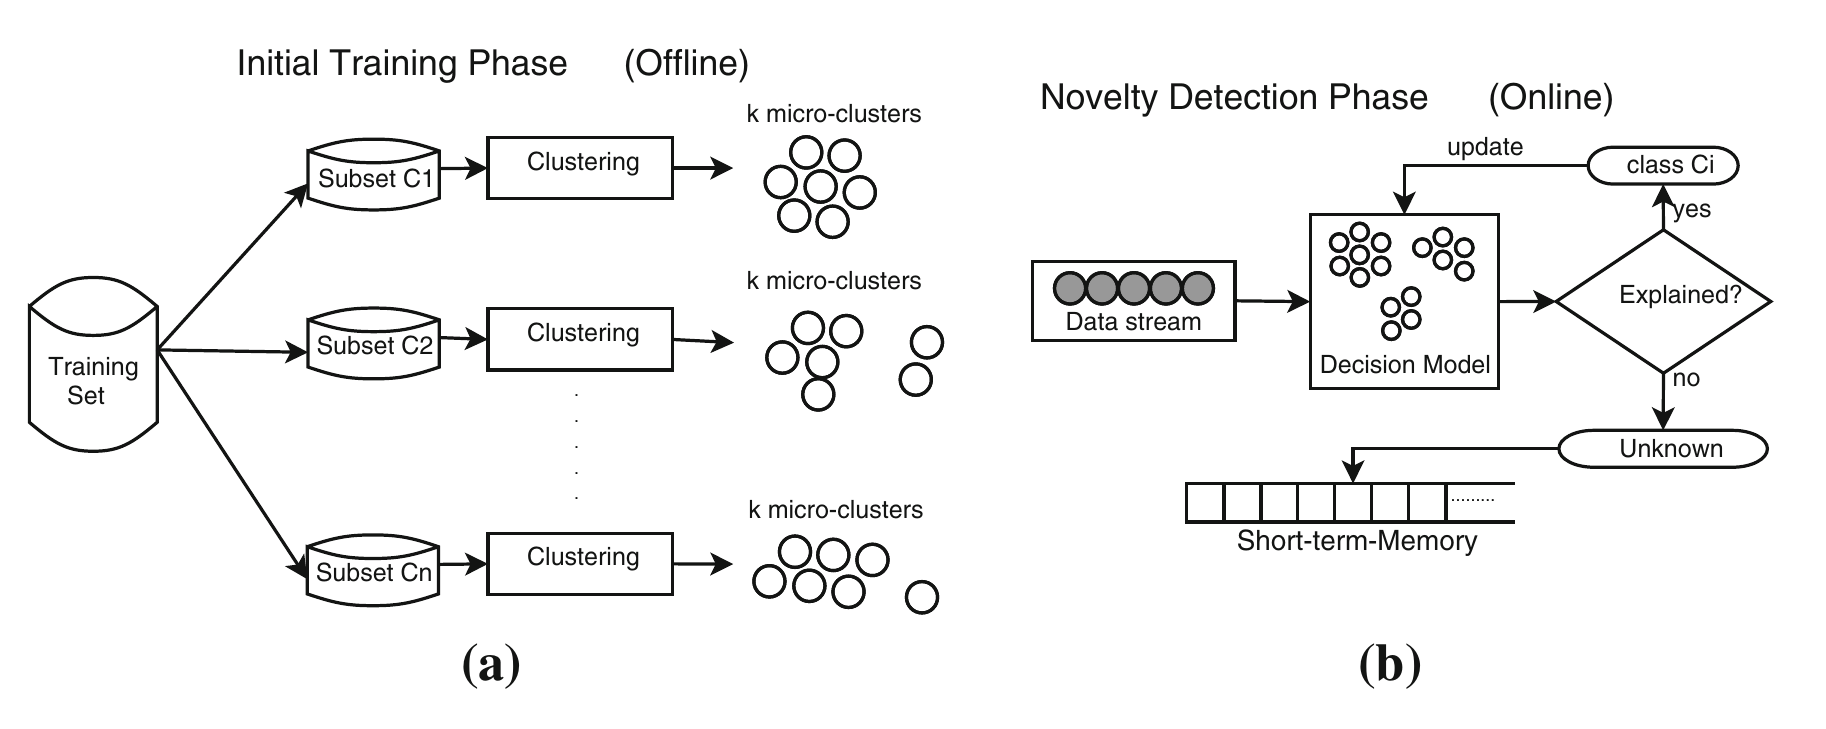
\includegraphics[width=\textwidth]{figuras/FariaMinas2015-fases.png}
  \caption{Visão geral do algoritmo MINAS com fases \emph{Offline} (a) e 
  \emph{Online} (b).}
  \fonte{\citeonline{Faria2016minas}.}
  \label{fig:minas}
\end{figure}
% \nota{Explique o desenho! o que significa cada objeto da figura? explique na figura.}
\end{frame}

\begin{frame}[fragile]{Fundamentos - \minas}
\begin{algorithm}[H]
  \SetKwFunction{nearestCluster}{clusterMaisPróximo}
  \SetKwFunction{NoveltyDetection}{DetecçãoNovidade}
  \SetKwFunction{handleModelSleep}{moveModeloAntigo}
  \SetKwFunction{removeOldSamples}{removeExemplosAntigos}
  % 
  \SetKwProg{Function}{Função}{:}{}
  \SetKwData{cleaningWindow}{janelaLimpeza}
  \SetKwData{noveltyDetectionTrigger}{gatilhoDetecçãoNov}
  \SetKwFunction{MinasOnline}{MinasOnline}
  % 
  \Function{\MinasOnline{Modelo, fluxoEntrada, fluxoSaída, \cleaningWindow, \noveltyDetectionTrigger}}{
    Desconhecidos $\leftarrow$ $\emptyset$; ModeloAntigo $\leftarrow$ $\emptyset$; últimaLimpeza $\leftarrow 0$; proximaNovidade $\leftarrow 0$\;
    \ForEach{ {$exemplo_{i}$} $\in$ fluxoEntrada }{
      % exemplo.rótulo $\leftarrow$ unknown\;
      % (distância, cluster) $\leftarrow$ \nearestCluster(exemplo, Modelo)\;
      maisPróximo $\leftarrow$ \nearestCluster(exemplo, Modelo)\;
      \eIf{maisPróximo.distância $<$ maisPróximo.cluster.raio}{
        exemplo.rótulo $\leftarrow$ maisPróximo.cluster.rótulo\;
        maisPróximo.cluster.últimoUso $ \leftarrow i$\;
      }
      {
        exemplo.rótulo $\leftarrow$ ``desconhecido''\;
        Desconhecidos $\leftarrow$ Desconhecidos $\cup$ exemplo\;
        \If{$|\;Desconhecidos\;| \geq$ \noveltyDetectionTrigger}{
          Modelo $\leftarrow$ Modelo $\cup$ \NoveltyDetection(Modelo $\cup$ ModeloAntigo, *Desconhecidos)\;
        }
        \If{ $ i > $ ( últimaLimpeza $ + $ \cleaningWindow )}{
          Modelo $\leftarrow$ \handleModelSleep(Modelo, *ModeloAntigo, últimaLimpeza)\;
          Desconhecidos $\leftarrow$ \removeOldSamples(Desconhecidos, últimaLimpeza)\;
          últimaLimpeza $ \leftarrow i $\;
        }
      }
      fluxoSaída.adicione(exemplo)\;
    }
  }
  \caption{Interpretação do algoritmo \minas \emph{online} \cite{Faria2016minas}.}
\label{alg:minas-main}
\end{algorithm}
\end{frame}

\begin{frame}[fragile]{Fundamentos - Processamento Distribuído de Fluxos}
    \begin{columns}[T,onlytextwidth]
      \column{0.5\textwidth}
        \vspace{1em}
        \begin{itemize}%[<+- | alert@+>]
          \item Arquiteturas \emph{Lambda} e \emph{Kappa};
          \item Mineração de Dados:
          \begin{itemize}
            \item \emph{MapReduce} e \emph{Apache Hadoop};
            \item \emph{Apache Spark} com \emph{Resilient Distributed Dataset - RDD};
          \end{itemize}
          \item Mineração de Fluxo de Dados:
          \begin{itemize}
            \item \emph{Apache Spark Streaming} com estratégia de \emph{micro-batching};
            \item \emph{Apache Storm};
            \item \emph{Apache Flink};
          \end{itemize}
          \item Não especializadas em fluxo de dados:
          \begin{itemize}
            \item Não-plataforma (construção dos mecanismos de envio e recebimento);
            \item Interface de Troca de Mensagens - MPI;
          \end{itemize}
        \end{itemize}
      \column{0.05\textwidth}
      \column{0.45\textwidth}
        % \vspace{-3em}
        \begin{figure}
          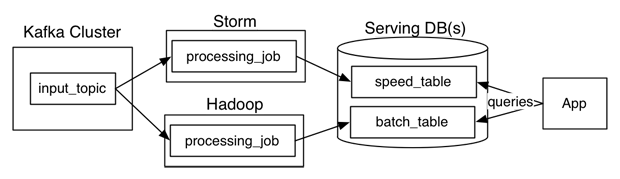
\includegraphics[width=\textwidth]{figuras/lambda.png}
          \caption{Arquitetura \emph{Lambda} com Kafka, Storm, Hadoop, SGBD tradicional e aplicação consumidora.}
          \fonte{\citeonline{Kreps2014}.}
        \end{figure}
        \vspace{-1em}
        \begin{figure}
            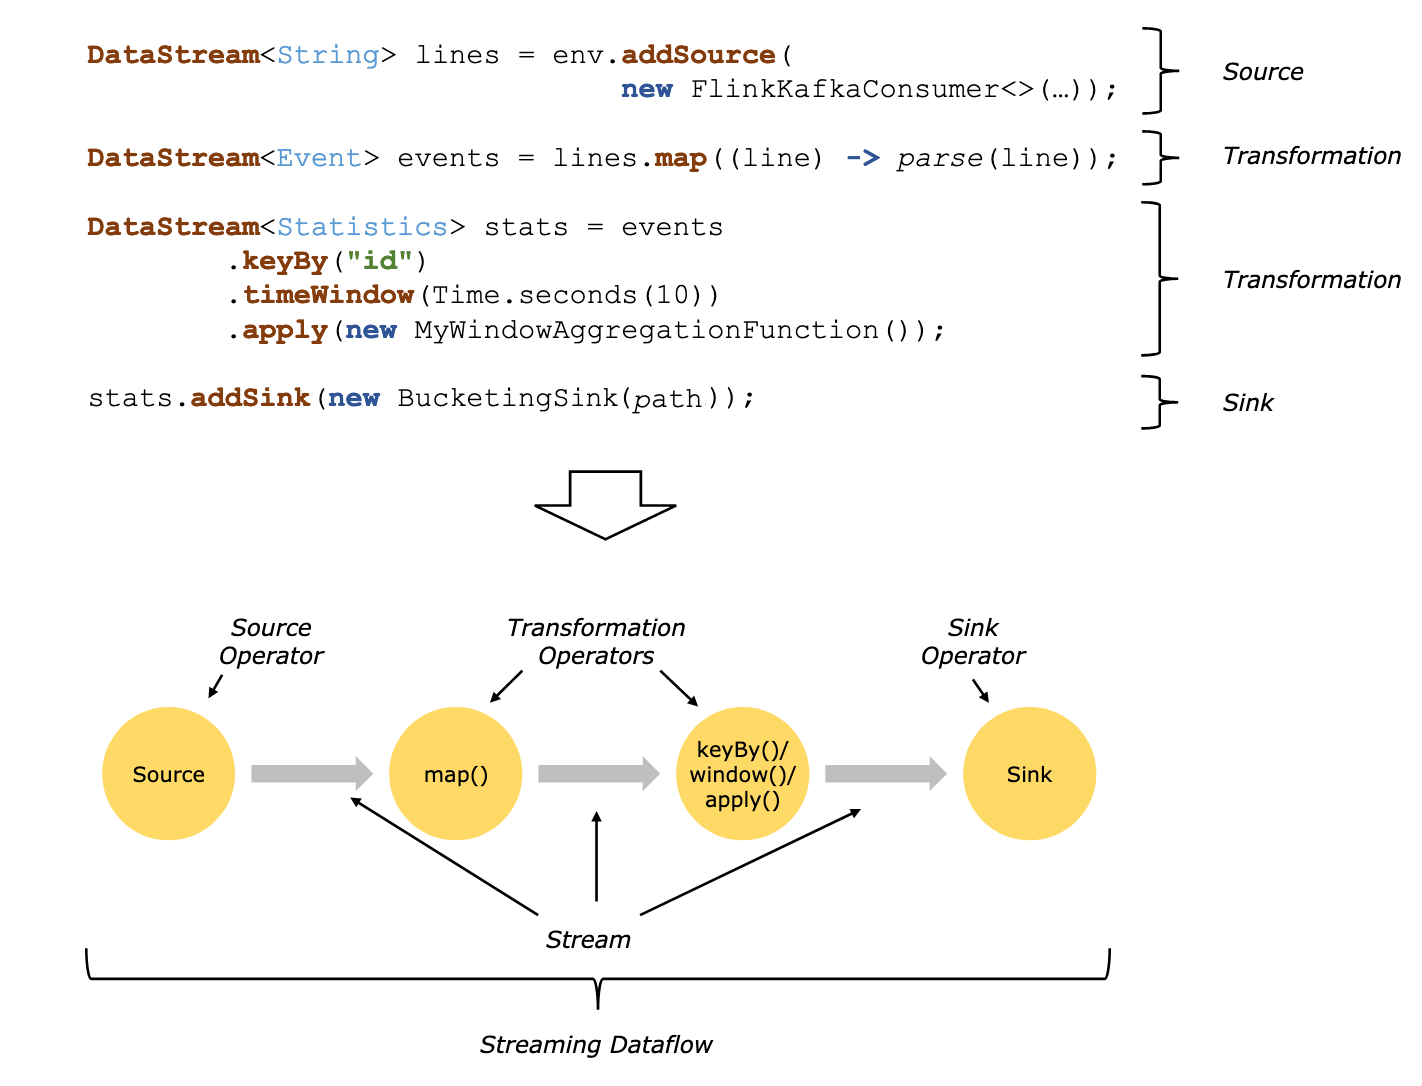
\includegraphics[width=\textwidth, trim={2cm 0 10cm 20cm},clip]{figuras/dataflow-code-flink.png}
            \caption{Arquitetura Apache Flink.}
            \fonte{\citeonline{ApacheFlink2020}.}
        \end{figure}
    \end{columns}

  % \nota{Faltou definir antes o que é processamento de fluxo.\\
  % \textbf{fluxo vs lote} deixar mais claro a diferença}

  % \nota{O slide fala de plataformas, mas vc falou de kappa e lambda
  % que não deveria falar neste slide}

  % \nota{Muita fala p/ esse slide (ficou explicando cada fundamento).
  % Deveria quebrar o slide em 3 ou 4 slides ao menos.}
\end{frame}

\begin{frame}[fragile]{Fundamentos - MPI}
  \begin{itemize}%[<+- | alert@+>]
    \item Localidade de dados;
    \begin{itemize}
      \item Menor número de \emph{page-faults} mantendo o Modelo em cache;
    \end{itemize}
    \item Memória distribuída e troca de mensagens;
    \item Padrão MPI - \emph{Message Passing Interface};
    \begin{itemize}
      \item Padrão MPI-4.0 aprovado pelo MPI Forum em 9 de Junho de 2021;
      \item Bibliotecas bem estabelecidas;
      \item Pares de operações \emph{send/receive}, entre outras operações;
      \item Execução gerenciada (\emph{Runtime Environment}, \texttt{mpirun});
    \end{itemize}
    \item Técnica SPMD - \emph{Single Program Multiple Data};
    \begin{itemize}
      \item Construção e execução simplificadas;
    \end{itemize}
  \end{itemize}
\end{frame}

\begin{frame}[fragile]{Fundamentos - Ambientes}
\begin{alertblock}{Ambientes de computação Distribuída}
\begin{itemize}
  \item Computação em Nuvem (\emph{Cloud Computing}) é um modelo que permite
  acesso conveniente a recursos computacionais compartilhados \cite{NIST2011}
  \begin{columns}[T,onlytextwidth]
    \column{0.5\textwidth}
    \begin{itemize}
      \item \textbf{Características Essenciais:}
      \begin{itemize}
        \item Auto-serviço sob demanda,
        \item Amplo acesso à rede,
        \item Agrupamento de recursos,
        \item Rápida elasticidade,
        \item Serviço mensurado;
      \end{itemize}
    \end{itemize}
    \column{0.5\textwidth}
    \begin{itemize}
      % \item \textbf{Modelo de Serviço:} \emph{Software} (SaaS), Plataforma (PaaS), Infraestrutura (IaaS);
      % \item \textbf{Implementações:} privada, comunitária, pública, híbrida.
      \item \textbf{Modelo de Serviço:}
      \begin{itemize}
        \item \emph{Software} (SaaS),
        \item Plataforma (PaaS),
        \item Infraestrutura (IaaS),
      \end{itemize}
      \item \textbf{Implementações:}
      \begin{itemize}
        \item Nuvem privada,
        \item Nuvem comunitária,
        \item Nuvem pública,
        \item Nuvem híbrida.
      \end{itemize}
    \end{itemize}
  \end{columns}
\end{itemize}
\end{alertblock}
% \nota{Separar os items em bullets (sub-bullets)}
\end{frame}

\begin{frame}[fragile]{Fundamentos - Ambientes}
\begin{alertblock}{Ambientes de computação Distribuída}
\begin{itemize}
  \item Computação de Borda (\emph{Edge Computing}):
  \\ Refere-se a qualquer recurso computacional ou de rede entre os dispositivos
  de borda e centro de dados hospedados em nuvem \cite{Shi2016}.

  \item Computação em Névoa (\emph{Fog Computing})
  
  % \cite{Bonomi2012,dastjerdi2016}
  
  % A horizontal, system-level architecture that distributes
  % computing, storage, control and networking functions closer to
  % the users along a cloud-to-thing continuum.
  
  Uma arquitetura horizontal a nível de sistema que distribui funções de
  computação, armazenamento, controle e rede próximos aos usuários no espaço
  contínuo nuvem-coisa \cite{IEEECommunicationsSociety2018}.
  \textbf{Características:}
  % \hspace{0.2\textwidth}
  \begin{columns}
    \column{0.15\textwidth}
    \column{0.3\textwidth}
    \begin{itemize}
      \item Mobilidade,
      \item Heterogeneidade,
      \item Baixa Latência,
      \item Distribuição geográfica,
    \end{itemize}
    \column{0.4\textwidth}
    \begin{itemize}
      \item Alto número de nós,
      \item Interoperabilidade e federação,
      \item Uso de fluxo de dados e aplicações em tempo real.
    \end{itemize}
    \column{0.15\textwidth}
  \end{columns}
  % \begin{block}{Características:}
  % \end{block}
\end{itemize}
\end{alertblock}
\end{frame}

% ------------------------------------------------------------------------------
\section{Estado da Arte e Trabalhos Relacionados}

\newcommand{\arch}{IDSA-IoT\xspace}

\begin{frame}[fragile]{Estado da Arte e Trabalhos Relacionados}
\begin{alertblock}{Sistemas de detecção de intrusão em redes}
  \begin{itemize}
    \item Ferramenta BigFlow \cite{Viegas2019}:
    \begin{itemize}
      % \nota{% OK, isso é trabalho relacionado!\\
      % Dissecar melhor [bigflow, catraca, idsa-iot]\\
      % passar mais rápido, detalhar nos próximos.}
      % \nota{BigFlow usa stream mining?\\
      % - qual é a grande contribuição?\\
      % - qual é a limitação?}
      \item[$\boldsymbol{+}$] Integração da extração dos descritores de fluxo à emissão de alarmes;
      \item[$\boldsymbol{+}$] Capacidade de tratamento de grandes volumes;
      \item[$\boldsymbol{-}$] Atualização semanal com avaliação de um especialista;
      \item[$\boldsymbol{-}$] Execução somente em nuvem.
    \end{itemize}
    \item Ferramenta CATRACA \cite{Lopez2018,Sanz2018}:
    \begin{itemize}
      % \nota{catraca: contribuição? limitação?}
      \item[$\boldsymbol{+}$] Divisão em camadas alocadas em nuvem e névoa;
      \item[$\boldsymbol{+}$] Modelo de decisão baseado em árvore de decisão;
      \item[$\boldsymbol{-}$] Extração dos descritores de fluxo é feita em
      névoa, classificação e detecção é feita em nuvem.
    \end{itemize}
    \item Arquitetura \arch \cite{Cassales2019a}:
    \begin{itemize}
      \item[$+$] Avaliação do algoritmo MINAS, ECSMiner e AnyNovel;
      \item[$+$] Distribuição das tarefas em nuvem e névoa focada em IoT;
      \item[$-$] Implementação e detalhamento da arquitetura em aberto.
    \end{itemize}
  \end{itemize}
\end{alertblock}
\end{frame}

\begin{frame}[fragile]{Estado da Arte e Trabalhos Relacionados}
\begin{figure}[ht]
  \centering
  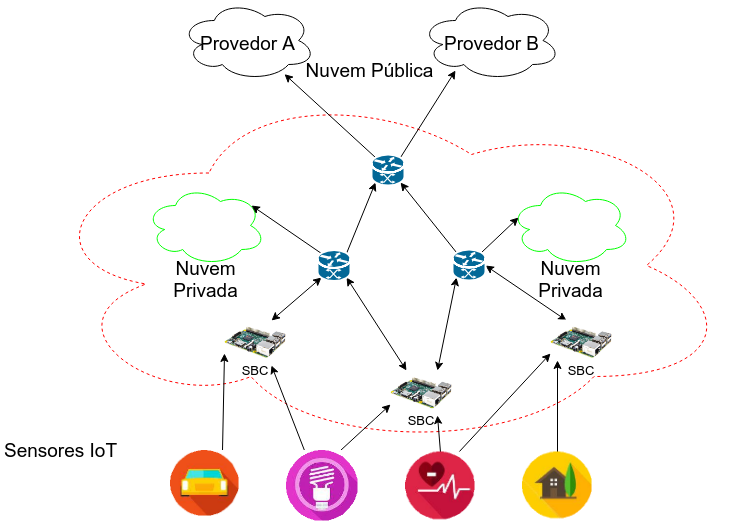
\includegraphics[width=0.48\textwidth]{figuras/idsa-iot-quali-000.png}
  \hfill
  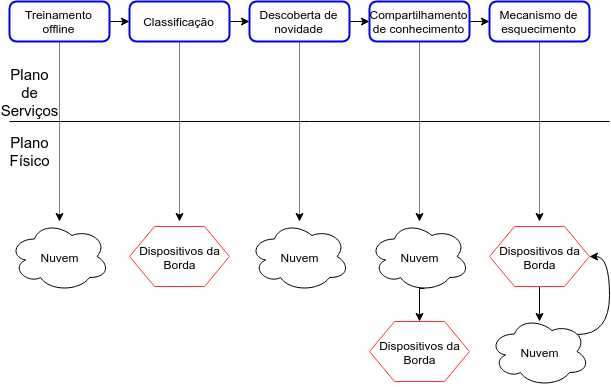
\includegraphics[width=0.48\textwidth]{figuras/idsa-iot-quali-004.png}
  \caption{Distribuição de serviços da arquitetura \arch.}
  \fonte{\citeonline{Cassales2019a}.}
  \label{fig:ids-iot}
\end{figure}
\end{frame}

% ------------------------------------------------------------------------------
\section{Proposta}

\newcommand{\mfog}{M-FOG\xspace}

\begin{frame}[fragile]{Proposta}
  \metroset{block=fill}
  \begin{block}{Pergunta de Pesquisa}
    \begin{itemize}
      \item É viável paralelizar e distribuir o algoritmo MINAS seguindo a arquitetura \arch?
      \item Quais são os efeitos na qualidade de classificação paralelizar e
      distribuir o algoritmo MINAS?
      
      % Proposta
      % \item Um sistema para detecção de intrusão em Redes IoT implementando em névoa;

      % % hipótese
      % \item A hipótese do trabalho é que o algoritmo MINAS pode ser distribuído em
      % névoa reduzindo a latência e com sem redução na qualidade de classificação.

      % \nota{pode falar:\\
      % - dificuldade de atualização de SW\\
      % - como foi o ataque MIRAI? (só curiosidade)\\
      % - capacidade de autodefesa? mesmo outros computadores não têm...}
    \end{itemize}
  \end{block}
\end{frame}

\begin{frame}[fragile]{Proposta}
  \metroset{block=fill}
  \begin{block}{Proposta da Pesquisa}
    \begin{itemize}
      
      \item Implementar a distribuição do algoritmo MINAS em nuvem e névoa
      conforme arquitetura \arch;
      
      \item Paralelizar o método de classificação do algoritmo MINAS.
    \end{itemize}
  \end{block}

  \metroset{block=transparent}
  \begin{alertblock}{Método}
    \begin{itemize}%[<+- | alert@+>]
      \item Plataforma de processamento distribuído;
      \item Estratégias de implementação da arquitetura \arch;
      \item Experimentação com a distribuição do algoritmo MINAS em ambientes;
      \item Métricas de qualidade de classificação para validação da implementação;
      \item Métricas de escalabilidade.
    \end{itemize}
  \end{alertblock}
  % \nota{Proposta\\
  % - poderia fazer algumas "perguntas" antes de fazer a sua proposta\\
  % => quais perguntas? (voce precisa saber quais)}
\end{frame}

\begin{frame}[fragile]{Proposta - Avaliações Preliminares}
  \begin{alertblock}{Primeira Implementação com \emph{Python} e \emph{Apache Kafka}}
    \begin{itemize}%[<+- | alert@+>]
      \item \emph{Python} é acessível e fornece bibliotecas diversas;
      \item \emph{Apache Kafka} é um sistema de mensagens distribuído;
      \begin{itemize}
        \item Interface de programação com cliente produtor e consumidor;
        \item Mensagens organizadas em tópicos que são distribuídos em partições;
      \end{itemize}
      \item A hipótese de que a carga seria distribuída entre os consumidores,
      uma vez que o consumidor pode selecionar uma partição para leitura;
      \item Em experimento com um produtor, 8 partições e 8 consumidores,
      observou-se que um consumidor processava a maior parte das mensagens,
      poucos consumidores recebiam algumas mensagens e a maioria dos consumidores
      não recebia mensagem alguma.
    \end{itemize}
  \end{alertblock}
% \nota{\textsc{cuidado,} o fato de vc não ter conseguido não significa que não é possível\\
% concluir que "o sistema não escala ..." (pode citar, só tome cuidado com a conclusão tirada)}
\end{frame}

\begin{frame}[fragile]{Proposta - Avaliações Preliminares}
  \begin{alertblock}{Segunda Implementação com \emph{Apache Flink}}
    \begin{itemize}%[<+- | alert@+>]
      \item Implementação escrita em Scala ou Java;
      \item Processamento de fluxos \emph{Stateful};
      \item Falta de bibliotecas que distribuam algoritmos base como \emph{K-means};
      \item Gerenciador de trabalhos (\emph{job manager}) e gerenciador de
      tarefas (\emph{job manager}) ocupam mais de $1\;GB$ em execuções
      consecutivas, portanto não é confiável para dispositivos pequenos.
    \end{itemize}
  \end{alertblock}
% \nota{métricas: Tem a fórmula? expressão?}
% \nota{"Avaliação do fluxo de saída do classificador" isto é uma métrica?}
% \nota{Incluir CR}
\end{frame}

\begin{frame}[fragile]{Proposta - Implementação MPI}
\begin{alertblock}{Terceira Implementação com MPI}
  \begin{itemize}
    \item Implementado em linguagem C, OpenMPI 4.0.4, seguindo a técnica SPMD;
    \item Dividido em 2 módulos e 4 tarefas.
    \item \texttt{mpirun} cria processos, o processo de \emph{0} executa o
    módulo raiz e os demais processos executam o módulo folha;
    \item Módulo raiz, com as tarefas \texttt{Fonte} e \texttt{Detector}, trata
    dos fluxos de entrada e saída além de gerenciar o conjunto de desconhecidos
    e a detecção de novidade;
    \item Módulo folha, com as tarefas \texttt{Classificador} e \texttt{Atualiza Modelo},
    trata da classificação de cada exemplo e manutenção do modelo local de cada instância.
  \end{itemize}
\end{alertblock}
\end{frame}

\begin{frame}[fragile]{Proposta - Implementação MPI}
  \begin{figure}[h]
    \centering
    \vspace{-0.5em}
    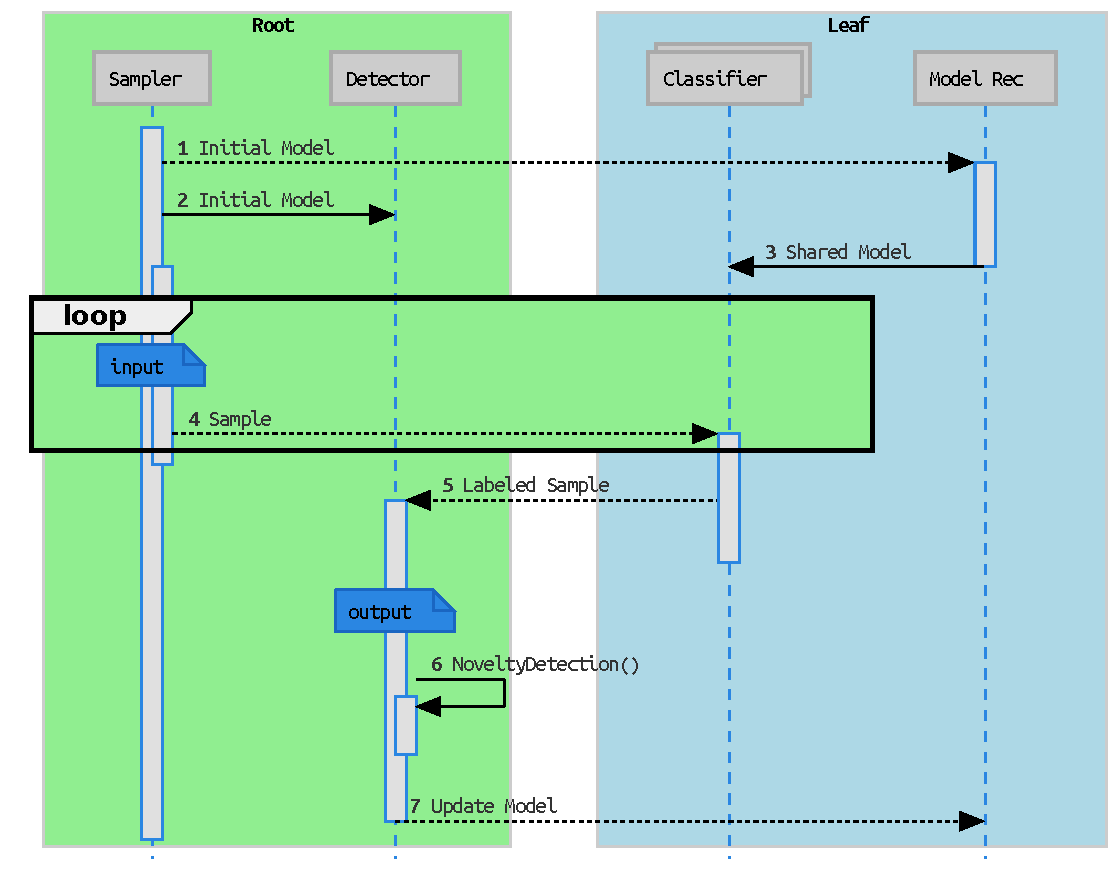
\includegraphics[width=0.8\textwidth,page=1]{figures/lifecycle-uml-svg.pdf}
    \vspace{-0.5em}
    \caption{Arquitetura e fluxos de dados do \mfog.}
    \vspace{-0.5em}
    \fonte{O autor.}
    \label{fig:arch}
  \end{figure}
\end{frame}

\begin{frame}[fragile]{Proposta - Método de Avaliação}
\begin{alertblock}{Métricas e Ambientes}
  \begin{itemize}
    \item Métricas de qualidade de classificação:
    \begin{itemize}
      \item Avaliação do fluxo de saída do classificador em uma matriz de confusão própria;
      \item Taxa de desconhecidos, acurácia e erro por classe.
    \end{itemize}
  \end{itemize}
\end{alertblock}
% \vspace{-3em}
\hspace{-1cm}
{
\small
\begin{minipage}{.55\textwidth}
  \begin{align}
    \mathbf{C} &= \{ c_1, c_2, \cdots, c_m \}\\
    \mathbf{Y} &= \{ y_1, y_2, \cdots, y_k \}\\
    \mathbf{L} &= \{ l_1, l_2, \cdots, l_n \} = \mathbf{C}' \cup \{ \text{``-''} \} \cup \mathbf{Y}\\
    \mathbf{E}_x &= (e_{ij})\in \mathbb{N} ^{m\times n}\\
      % \mathbf{E}_x &= \begin{pmatrix}
      %   e_{1,1} & e_{1,2} & \cdots & e_{1,n} \\
      %   e_{2,1} & e_{2,2} & \cdots & e_{2,n} \\
      %   \vdots  & \vdots  & \ddots & \vdots  \\
      %   e_{m,1} & e_{m,2} & \cdots & e_{m,n} 
      % \end{pmatrix}\\
      A(l_j) &= \begin{cases} 
        %\downarrow 
        \nexists & \text{se } l_j = \text{``-''} \\
        c_i      & \text{se } \exists c_i = l_j \;: c_i \in \mathbf{C}' \\
        c_i      & \text{se } e_{ij} = max\{ e_{aj} : j \in [0, m] \}
      \end{cases}\\
      \mathit{UnkR}_{x, i} &= \frac{e_{i j} : l_j = \text{``-''}}{\sum_{j=1}^{n} e_{i j}}
  \end{align}
\end{minipage}%
\hspace{0.5cm}
\begin{minipage}{.45\textwidth}
  \begin{align}
    tp_i &= \sum_{j=1}^{n} e_{ij} \; \text{ se } l_j \neq \text{``-''} \text{ e } A(l_j) = c_i\\
    fn_i &= \sum_{j=1}^{n} e_{ij} \; \text{ se } l_j \neq \text{``-''} \text{ e } A(l_j) \neq c_i\\
    \mathit{acc}_x &= \frac{1}{m} \sum_{i=1}^{m} \frac{tp_i}{fn_i + tp_i}\\
    \mathit{err}_x &= \frac{1}{m} \sum_{i=1}^{m} \frac{fn_i}{fn_i + tp_i}%
  \end{align}%
\end{minipage}
}
\end{frame}

\begin{frame}[fragile]{Proposta - Método de Avaliação}
  \begin{alertblock}{Métricas e Ambientes}
    \begin{itemize}
      \item Métricas de escalabilidade:
      \begin{itemize}
        \item Número e tipo de processadores;
        \item Uso de memória;
        \item Tempo de processamento;
        \item Latência, tempo entre a entrada e saída de cada descritor de fluxo.
      \end{itemize}
      \item Ambientes de teste:
      \begin{itemize}
        \item Computador Pessoal (para desenvolvimento);
        \item Nevoa composta de SBC (\emph{Sigle Board Computer}) ARM 4 núcleos;
        \item Conjunto de dados para IDS, Kyoto 2006+, segmento dezembro de 2015
        como estabelecido por \citeonline{Cassales2019a}.
      \end{itemize}
    \end{itemize}
  \end{alertblock}
\end{frame}

\section{Resultados}

\newcommand{\expA}{\textit{a-Referência}\xspace}
\newcommand{\expB}{\textit{b-Sequencial}\xspace}
\newcommand{\expC}{\textit{c-Paralelo}\xspace}
\newcommand{\expD}{\textit{d-Distribuído}\xspace}
\begin{frame}[fragile]{Resultados - Experimentos}
    \begin{table}[htb]
      \centering
      \caption{Listagem dos principais experimentos.}
      \begin{tabular}{p{0.17\textwidth}|p{0.27\textwidth}|p{0.47\textwidth}}
      \textbf{Experimento} & \textbf{Programa}                 & \textbf{Características} \\\hline
      \expA                & \minas referência 2013            & Raio é a distância máxima. \\\hline
      \expB                & \minas sequencial para validação  & 
        Raio é o desvio padrão das distâncias;
        Modelo único;
        Remoção de desconhecidos mais agressivo. \\\hline
      \expC                & \mfog 1 nó, 4 processadores       & 
        Classificadores paralelos;
        Detecção de novidade assíncrona. \\\hline
      \expD                & \mfog 3 nós, 12 processadores     &
        Mais processadores;
        Comunicação em rede.
      \end{tabular}
    \end{table}
\end{frame}

\begin{frame}[fragile]{Resultados - Validação}
  \begin{figure}
    \begin{subfigure}{0.49\textwidth}
      \centering
      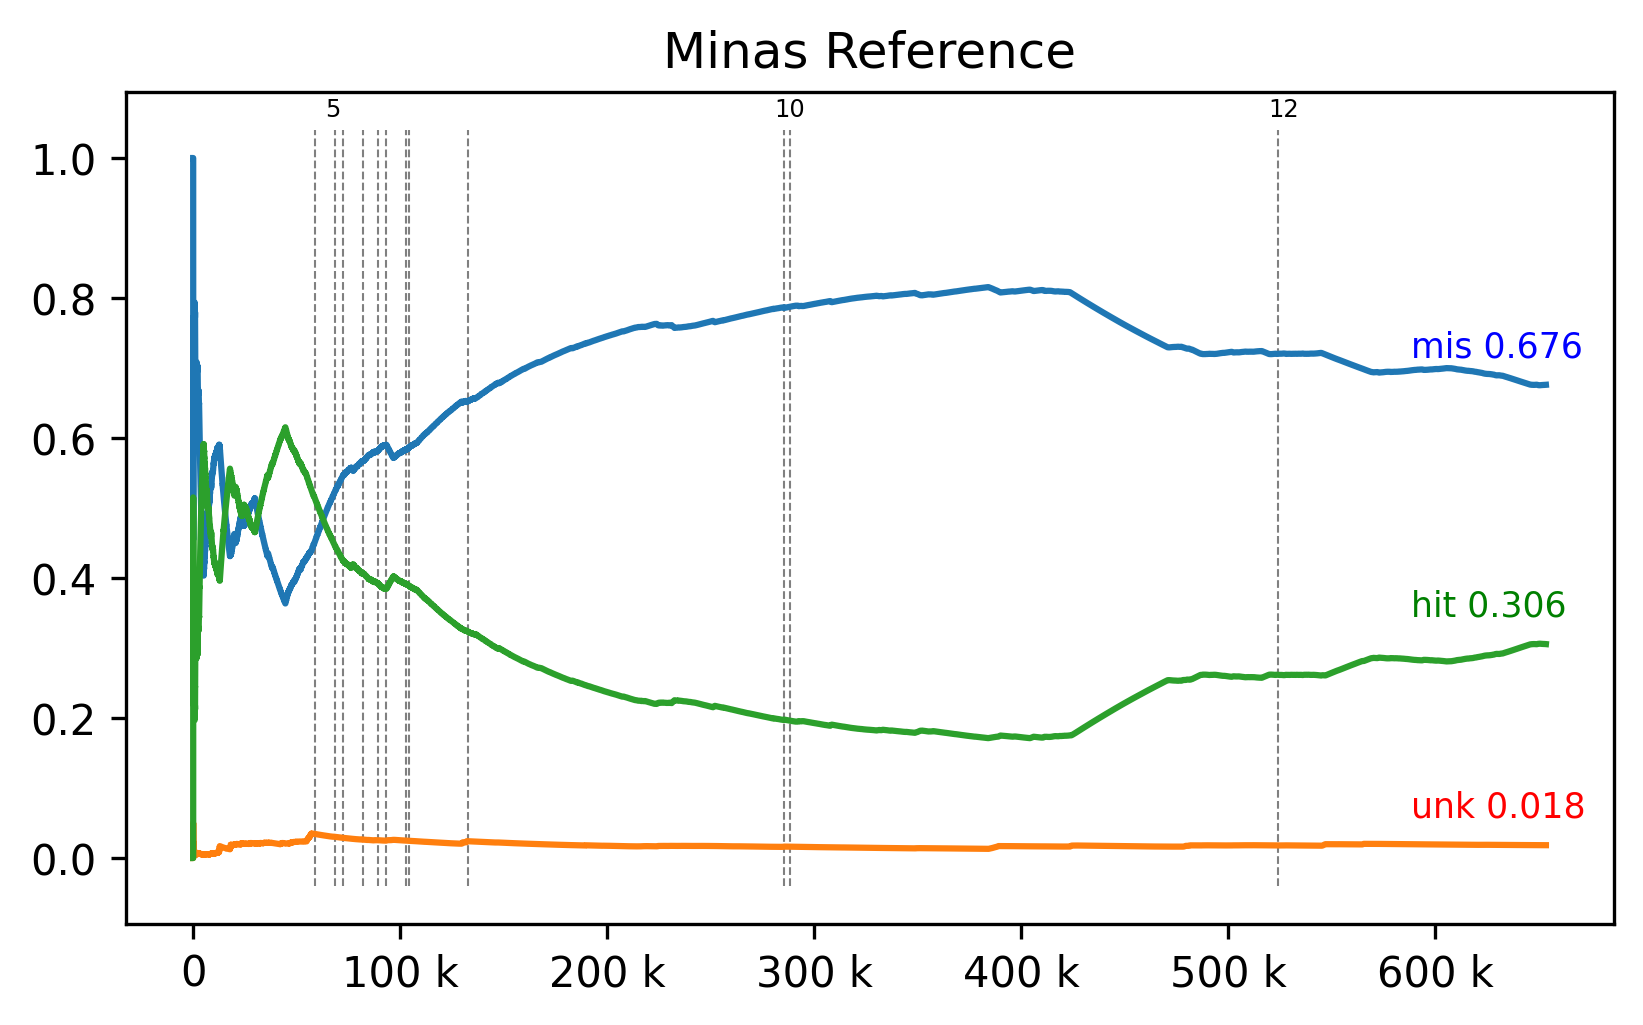
\includegraphics[width=1\linewidth]{experiments/revised-java-log.png}
      \caption{Experimento \expA, implementação de referência do algoritmo \minas.}
      \label{fig:validation-java}
    \end{subfigure}
    \hfill
    \begin{subfigure}{0.49\textwidth}
      \centering
      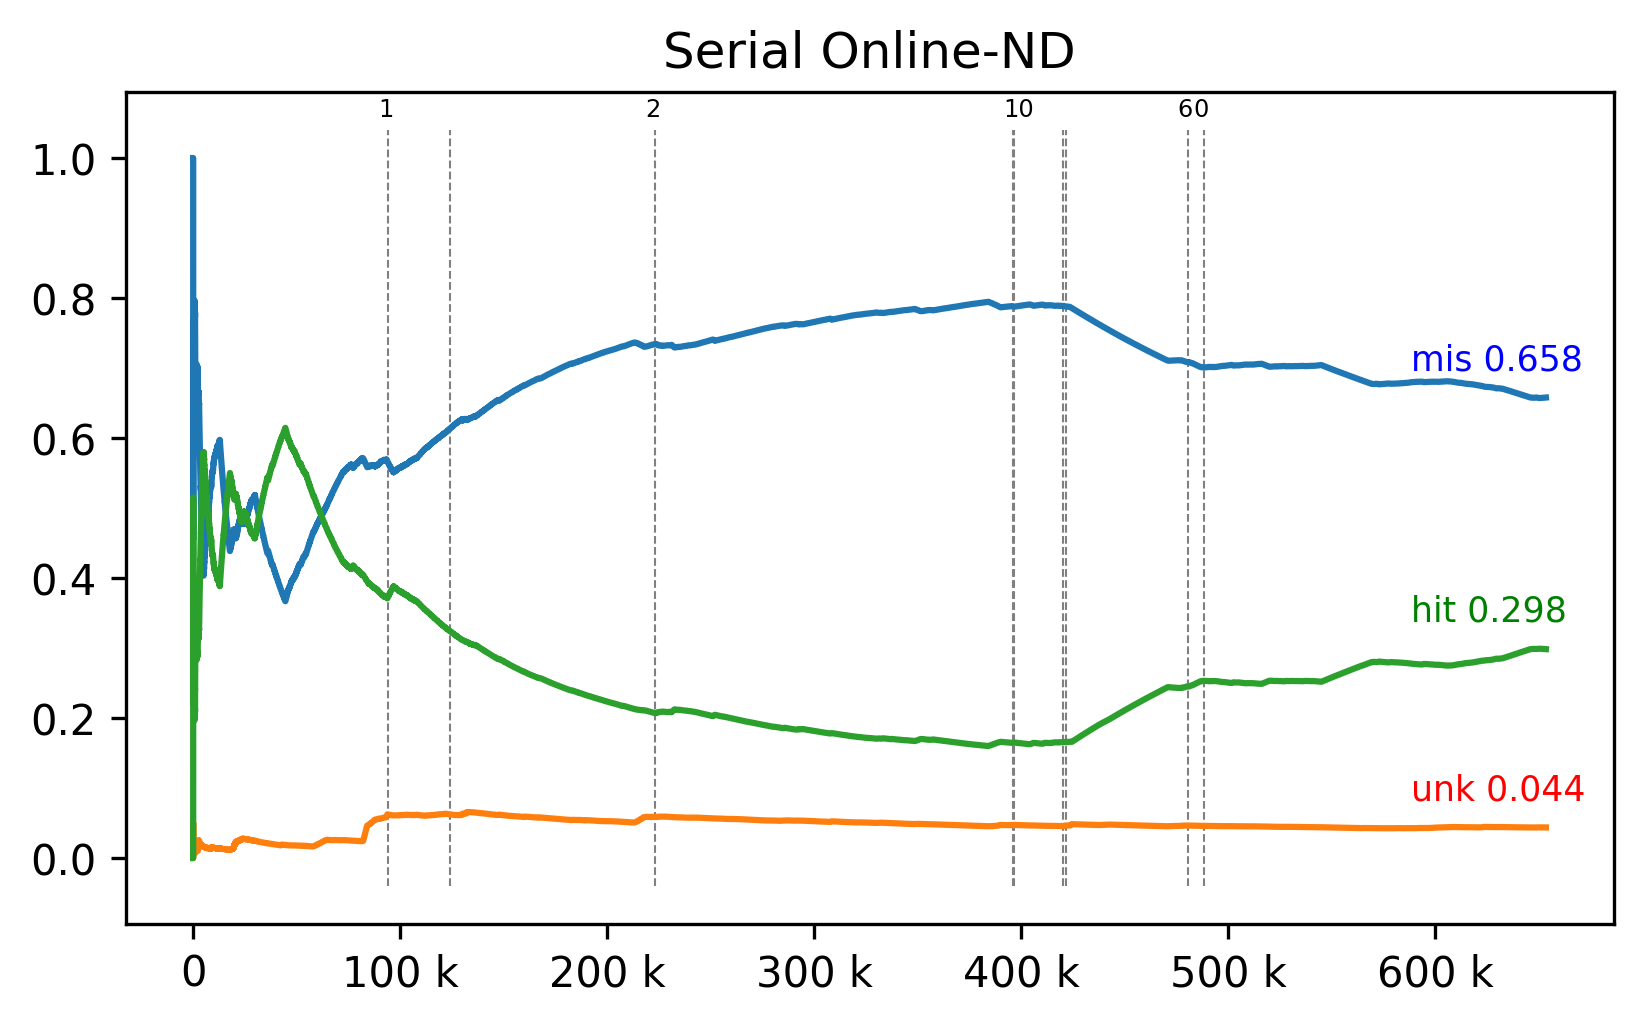
\includegraphics[width=1\linewidth]{experiments/online-nd-log.png}
      \caption{Experimento \expB, \mfog sequencial.}
      \label{fig:validation-serial}
    \end{subfigure}
    \caption{Visualização de fluxo do conjunto \emph{Kyoto} Dez. 2015.}
    \fonte{O autor.}
  \end{figure}
\end{frame}

\begin{frame}[fragile]{Resultados - Efeitos Distribuição}
  \begin{figure}
    \begin{subfigure}{0.49\textwidth}
      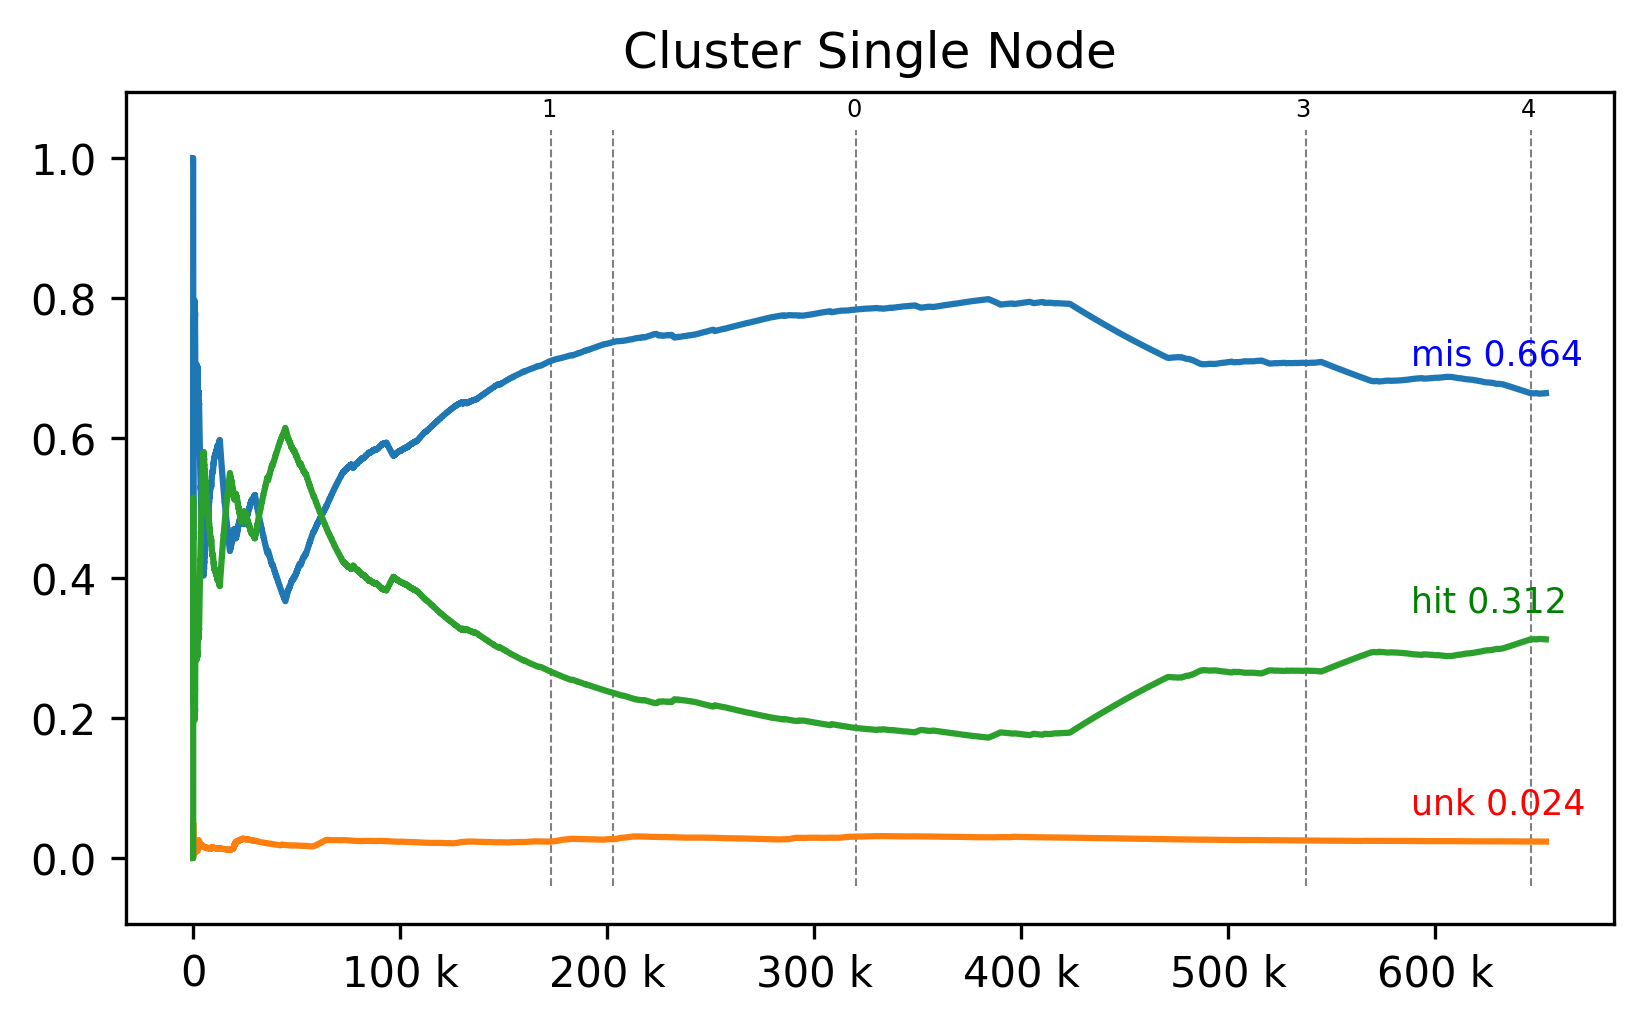
\includegraphics[width=1\linewidth]{experiments/tmi-base-log.png}
      \caption{Experimento \expC, \mfog com 1 nó e 4 núcleos.}
      \label{fig:single-flow}
    \end{subfigure}
    \hfill
    \begin{subfigure}{0.49\textwidth}
      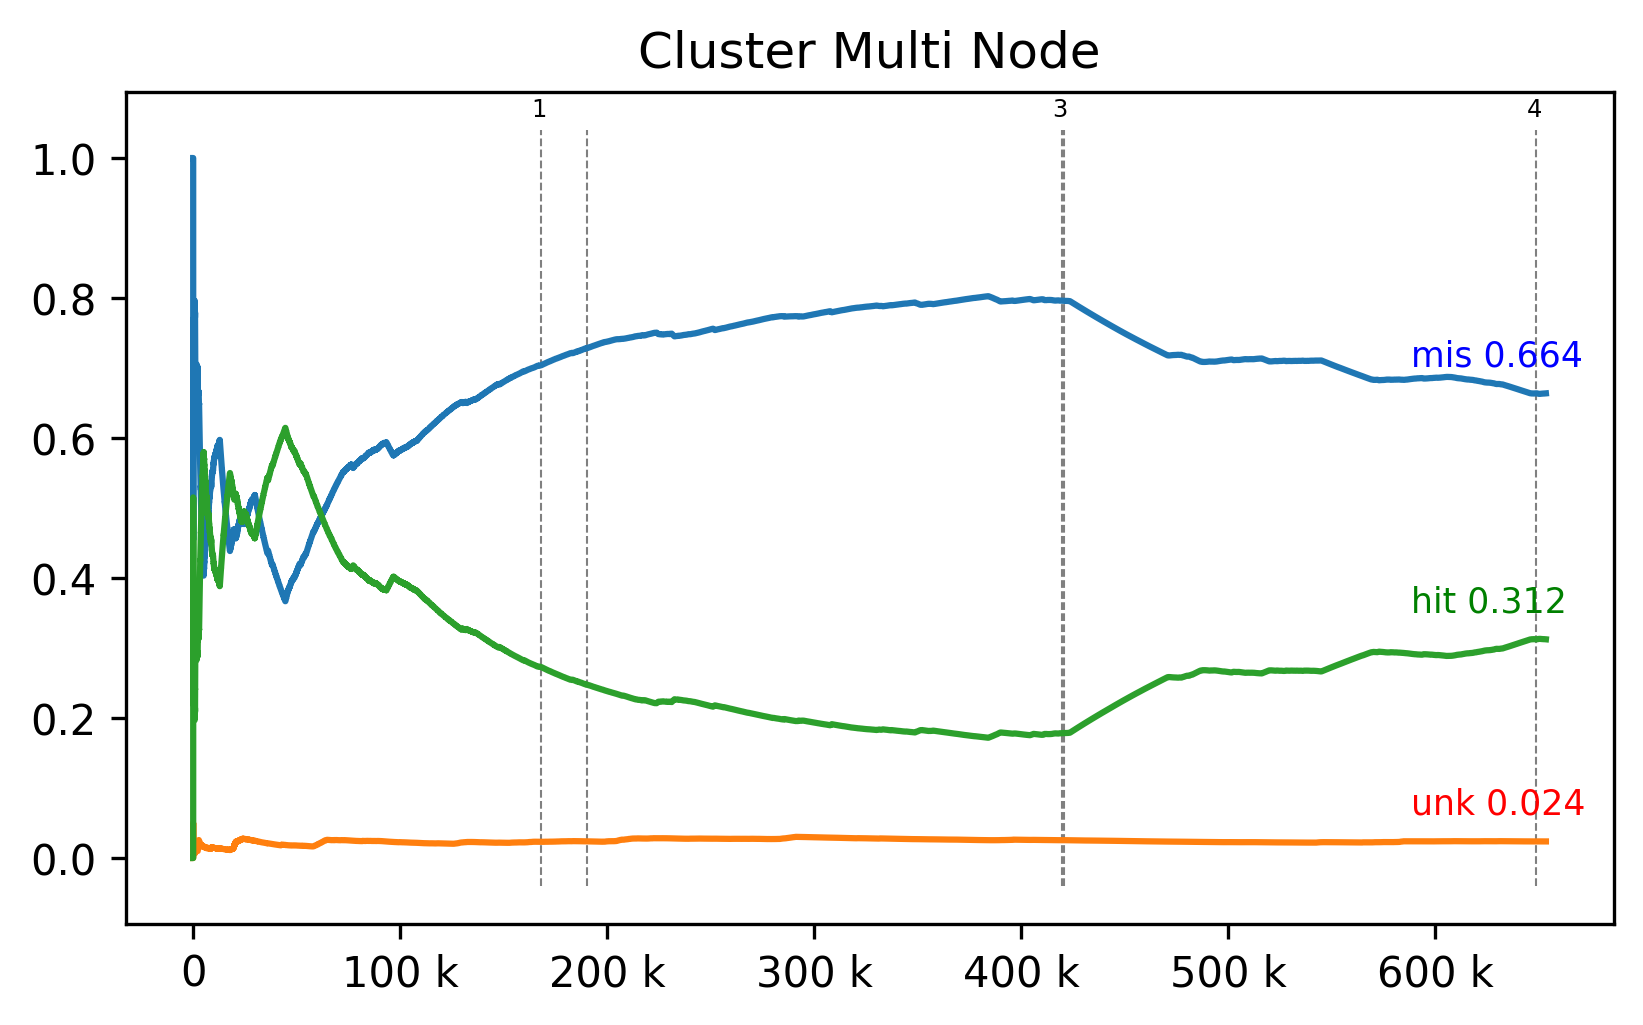
\includegraphics[width=1\linewidth]{experiments/tmi-n12-log.png}
      \caption{Experimento \expD, \mfog com 3 nós de 4 núcleos cada.}
      \label{fig:multi-flow}
    \end{subfigure}
    \caption{Visualização de fluxo do conjunto \emph{Kyoto} Dez. 2015.}
    \fonte{O autor.}
  \end{figure}
\end{frame}

\begin{frame}[fragile]{Resultados - Experimentos Principais}
  \begin{table}[hbt]
    \centering
    \caption{Sumário das métricas extraídas dos experimentos principais.}
    \begin{tabular}{l|r|r|r|r|r}
    Experimento     & \expA         & \emph{Offline} & \expB          & \expC       & \expD       \\
    Métrica         &               &               &                 &             &             \\\hline
    \texttt{unk}    & $0.018333$    &               & $0.043717$      & $0.023521$  & $0.023718$  \\\hline
    \texttt{hit}    & $0.305618$    &               & $0.298438$      & $0.312416$  & $0.312478$  \\\hline
    \texttt{err}    & $0.676049$    &               & $0.657843$      & $0.664061$  & $0.663802$  \\\hline
    Novidades       & $12$          &               & $9$             & $5$         & $5$         \\\hline
    Tempo     ($s$) & $2761.83$     & $194.12$      & $80.79$         & $522.10$    & $207.14$    \\\hline
    Sistema   ($s$) & $7.15$        & $ 0.075$      & $11.51$         & $ 47.77$    & $157.61$    \\\hline
    Decorrido ($s$) & $2772.07$     & $194.27$      & $93.03$         & $145.04$    & $ 95.38$    \\\hline
    Latência  ($s$) & $4.24\cdot10^{-3}$  &       & $1.42\cdot10^{-4}$  & $2.22\cdot10^{-4}$  & $1.46\cdot10^{-4}\ $  \\\hline
    Processadores   & $1$           &  $1$          &  $1$            & $4$         & $12$        \\\hline
    \emph{Speedup}  &               &               &                 & $0.6414092$ & $0.9753617$  \\\hline
    Eficiência      &               &               &                 & $0.1603523$ & $0.0812801$  
    \end{tabular}
  \end{table}
\end{frame}

\begin{frame}[fragile]{Resultados - Variação Processadores}
  \begin{figure}
    \centering
    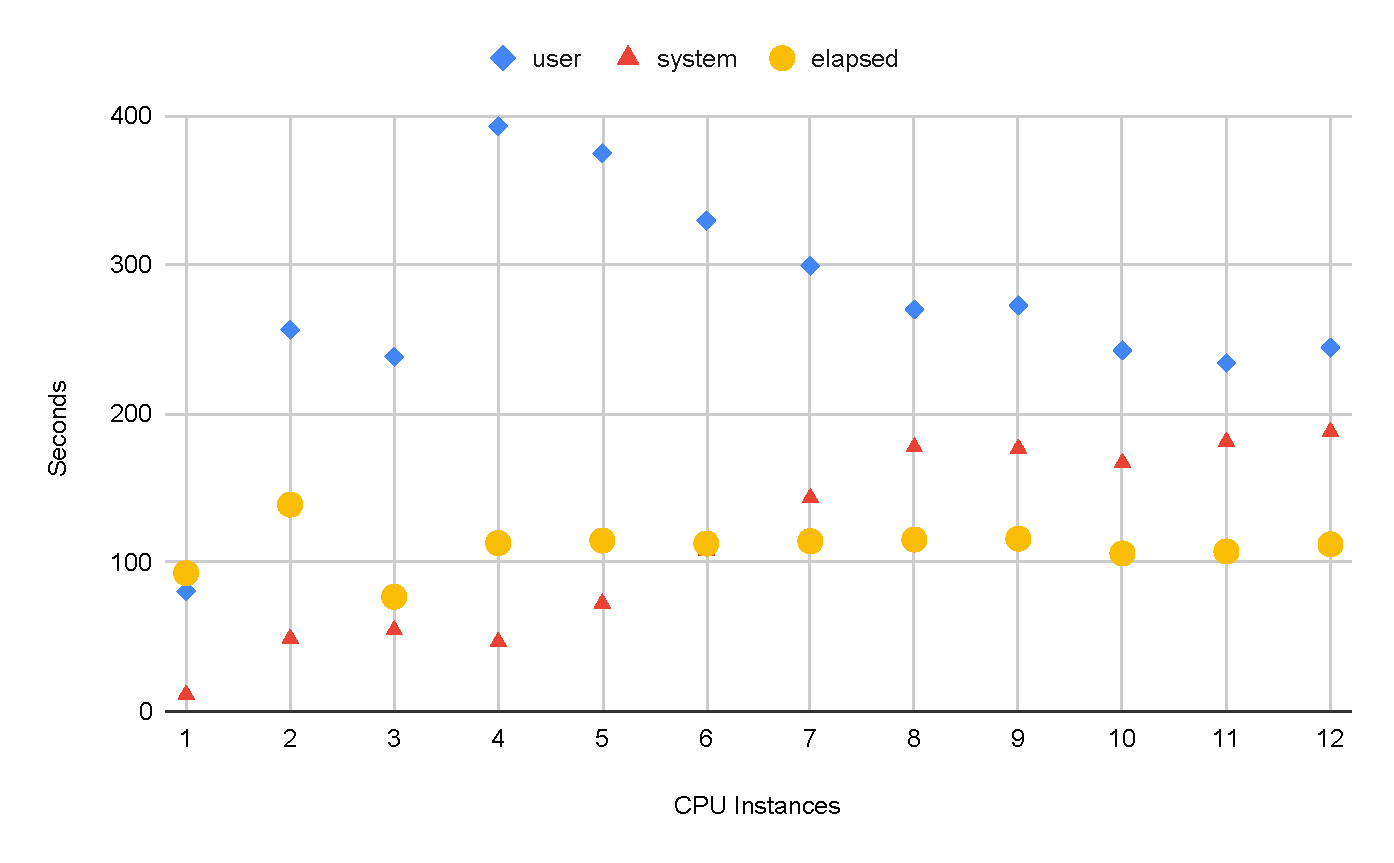
\includegraphics[width=0.7\linewidth,page=1]{experiments/speedup-clean.pdf}
    \caption{Métricas de tempo para execuções do \mfog com variação no número de processadores.}
    \label{fig:speedup}
    \fonte{O autor.}
  \end{figure}
\end{frame}

\begin{frame}{Resultados - Latência (i)}
  \begin{figure}[h]
    \centering
    \begin{subfigure}{0.49\textwidth}
      \centering
      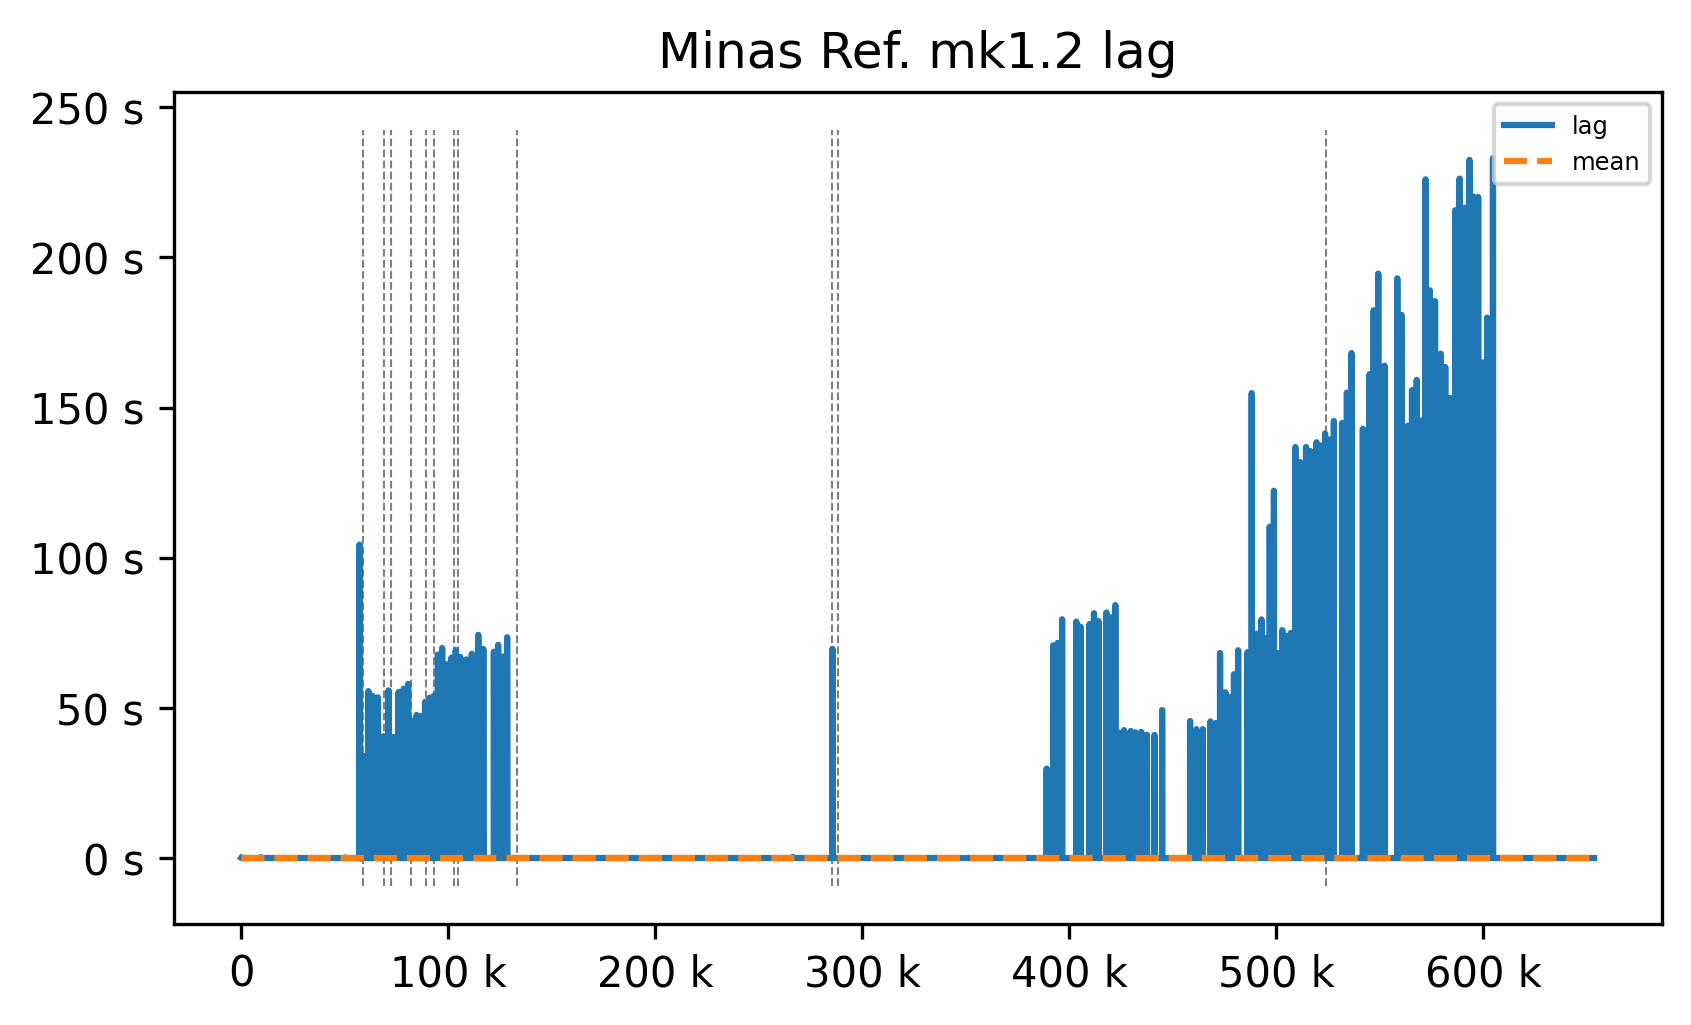
\includegraphics[width=1\linewidth]{experiments/lag-java.png}
      \caption{Implementação de referência.}
    \end{subfigure}
    \hfill
    \begin{subfigure}{0.49\textwidth}
      \centering
      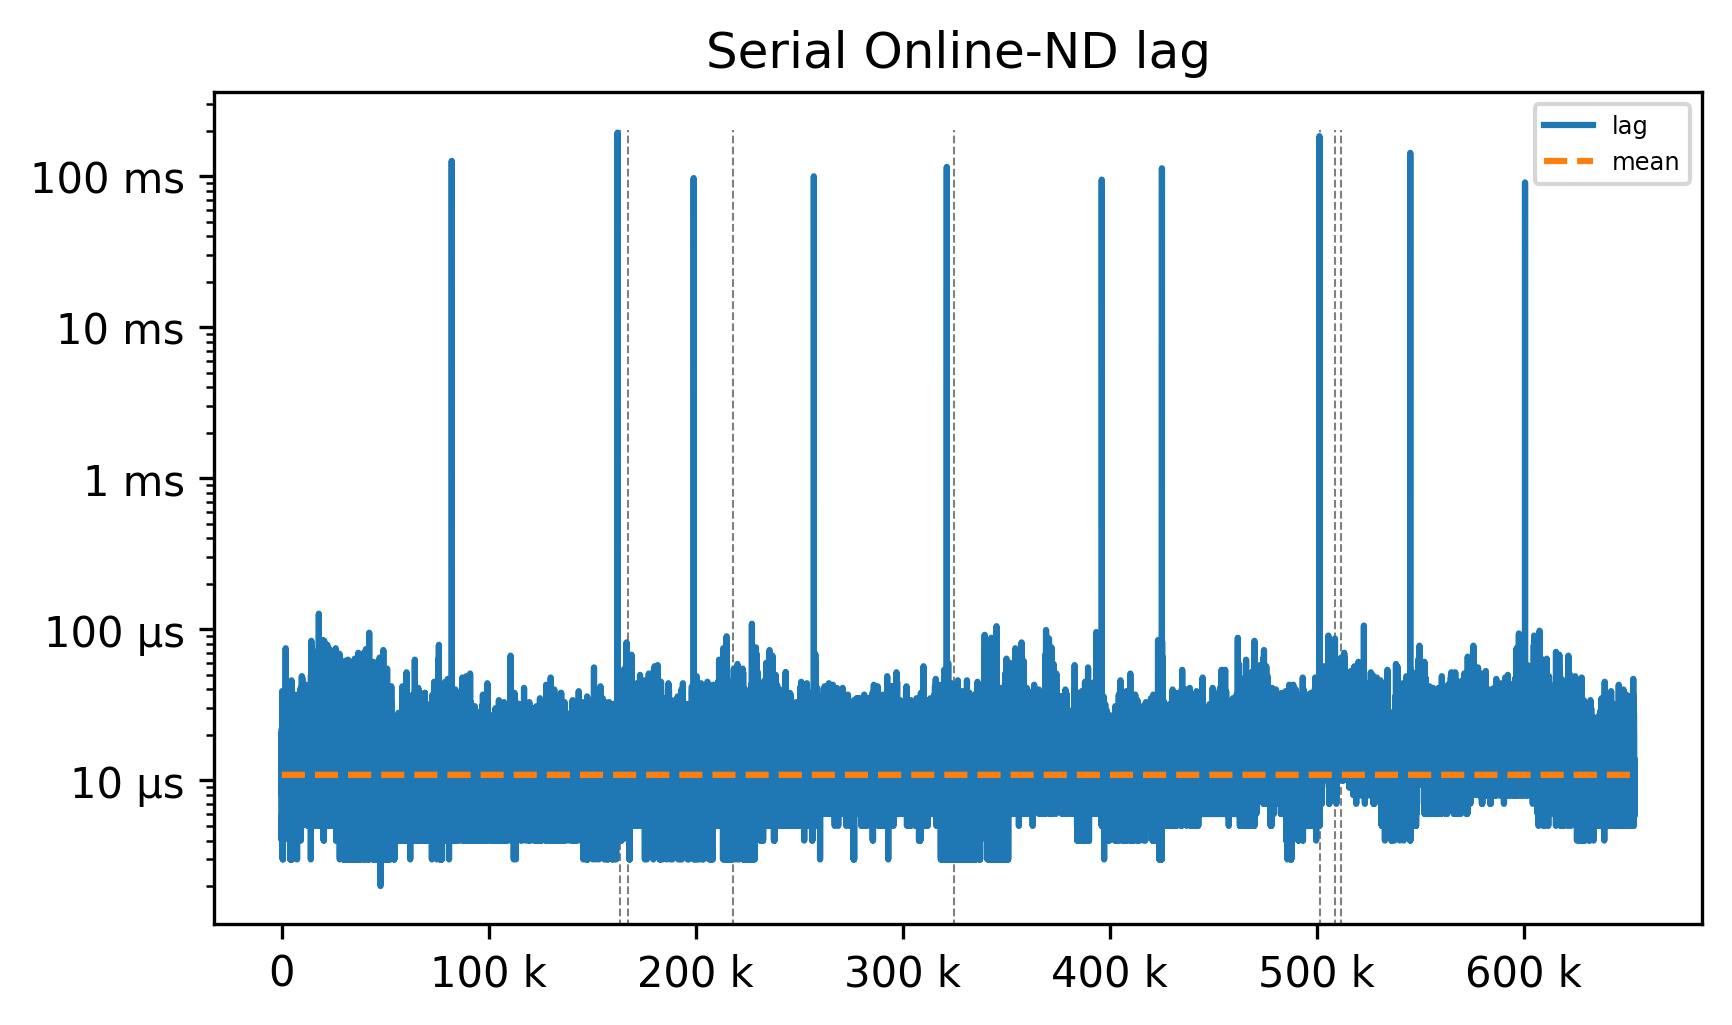
\includegraphics[width=1\linewidth]{experiments/lag-serial.png}
      \caption{Implementação sequencial.}
    \end{subfigure}
    \caption{Visualização de Latência.}
    \fonte{O autor.}
  \end{figure}
\end{frame}
\begin{frame}{Resultados - Latência (ii)}
    \begin{figure}[h]
      \centering
      \begin{subfigure}{0.7\textwidth}
        \centering
        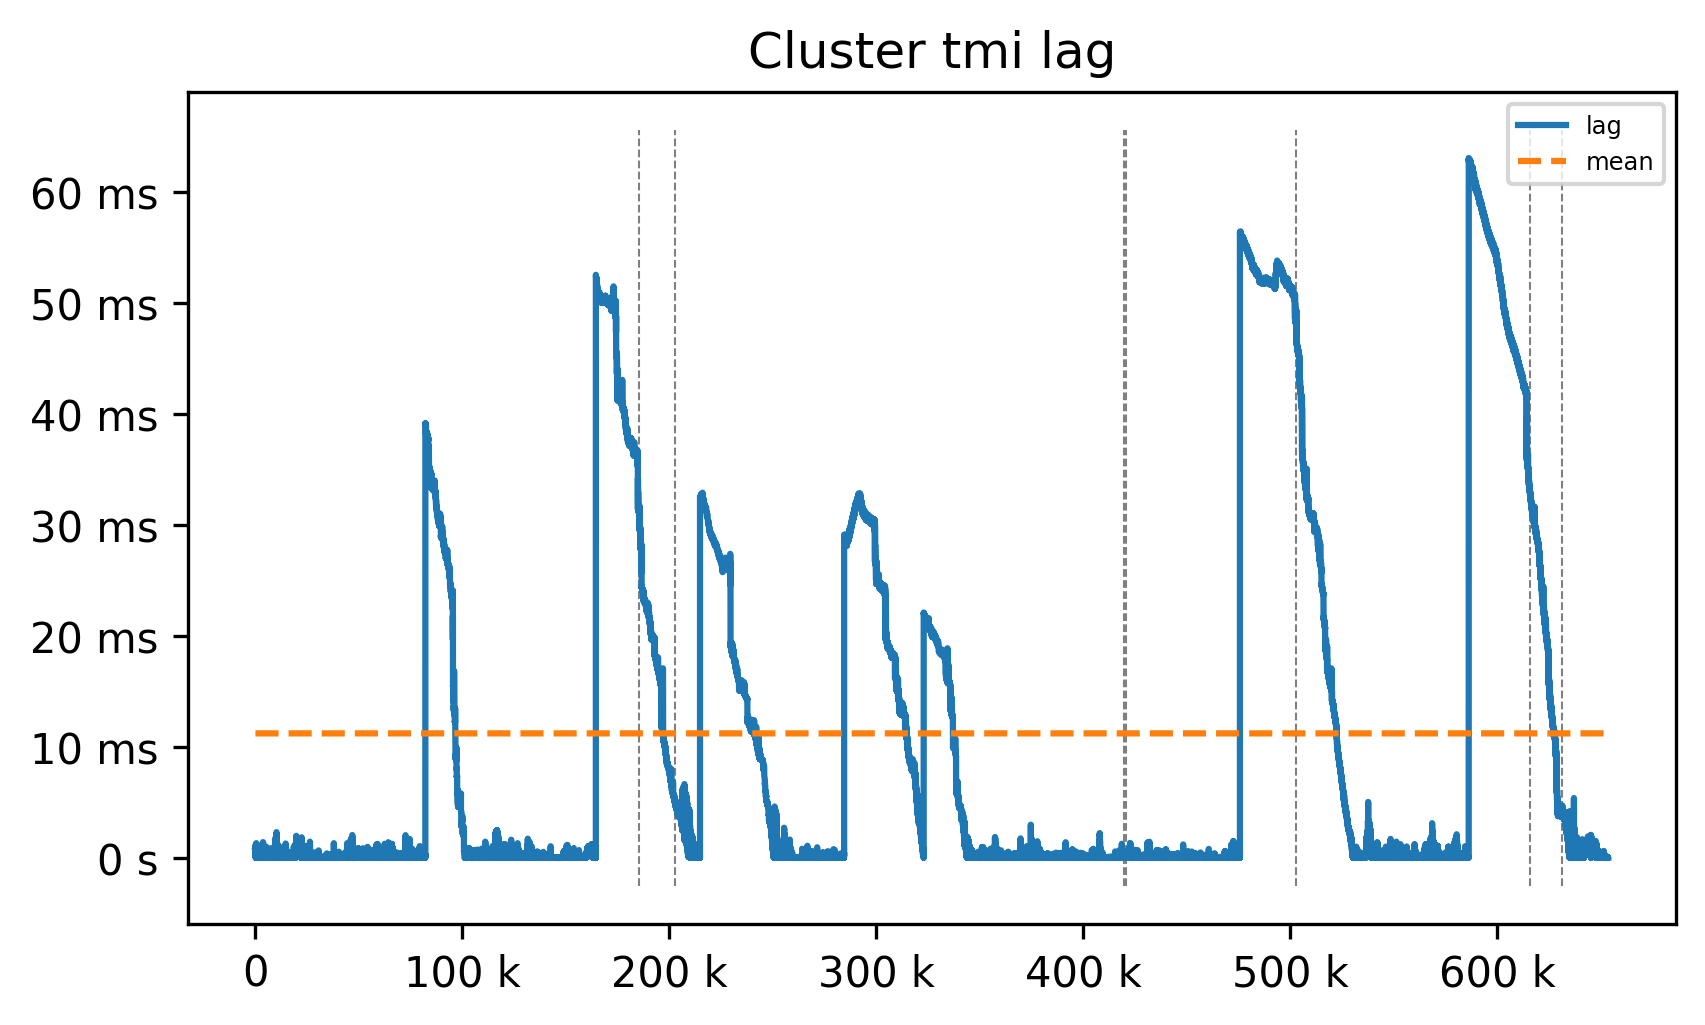
\includegraphics[width=1\linewidth]{experiments/lag-mfog.png}%
        \addtocounter{figure}{-1}\addtocounter{subfigure}{2}%
        \caption[label=c]{Implementação paralela.}%
      \end{subfigure}
      \caption{Visualização de Latência.}
      \fonte{O autor.}
    \end{figure}
\end{frame}

\section{Conclusão}
\begin{frame}{Conclusão}
  
  \begin{alertblock}{Resultados obtidos:}
  \begin{itemize}
    \item Algoritmo \minas distribuído e a arquitetura \arch
    implementada com modificações;
    \item Distribuição tem pequeno efeito sobre as métricas de qualidade;
    \begin{itemize}
      \item Maior efeito é a redução de etiquetas novidade na versão distribuída;
    \end{itemize}
    \item Resultados mostram que a implementação \mfog não atinge escala pelo CCR e eficiência;
  \end{itemize}
  \end{alertblock}
  
  \vspace{.5em}
  \begin{alertblock}{Trabalhos futuros:}
  \begin{itemize}
    \item Da arquitetura: Distribuição do modelo entre redes distintas (conjuntos aditivos);
    \item Na implementação:
    \begin{itemize}
    \item Outros algoritmos de agrupamento (CluStream);
    \item Estratégia de otimização da distribuição de carga (micro ou mini batching);
    \item Outras plataformas de processamento otimizadas para o ambiente névoa;
    \end{itemize}
    \item No algoritmo:
    \begin{itemize}
    \item Explorar distribuição espacial dos clusters (polígonos sem
    sobreposição, árvore de busca);
    \item Algoritmo com modelo de tamanho fixo (máxima precisão com recursos disponíveis);
    \end{itemize}
  \end{itemize}
  \end{alertblock}
\end{frame}

\begin{frame}{Contribuições e Publicações}
  \begin{itemize}
    
    \item Artigo aceito na seção geral da 21ª Conferência Internacional em
    Computação Ciêntífica e suas Aplicações (ICCSA 2021,
    \url{https://iccsa.org/}) em Cagliari, Itália, Setembro 13-16 2021
    \cite{Puhl2021};
    
    % July 5-8, 2021: ICCSA 2021 Conference
    % September 13-16, 2021: ICCSA 2021 Conference
    
    \item Código fonte com experimentos e métodos publicamente disponíveis em
    \url{https://github.com/luis-puhl/minas-flink}.
  
  \end{itemize}
\end{frame}

{\setbeamercolor{palette primary}{fg=black, bg=yellow}\begin{frame}[standout]
  Obrigado!
\end{frame}}

\begin{frame}[allowframebreaks]{Referências}
  \bibliography{99.referencias.bib}
\end{frame}

\appendix

% \begin{frame}[fragile]{Extra}
%   \begin{figure}[ht]
%     \centering
%     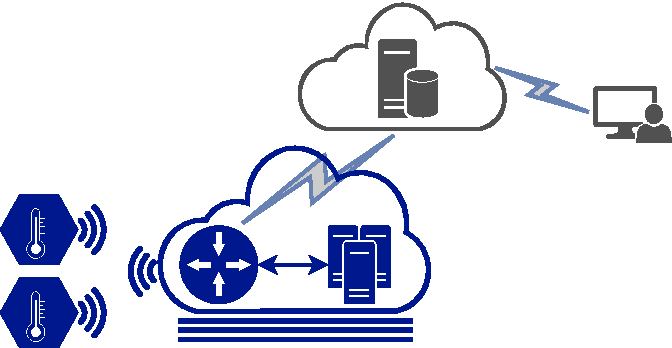
\includegraphics[width=0.8\linewidth]{figures/mfog-arch-fisica.svg.pdf}
%     \caption{Arquitetura IoT tradicional.}
%     \fonte{O autor.}
%     \label{fig:ids-iot-phy}
%   \end{figure}
% \end{frame}
\begin{frame}\centering
  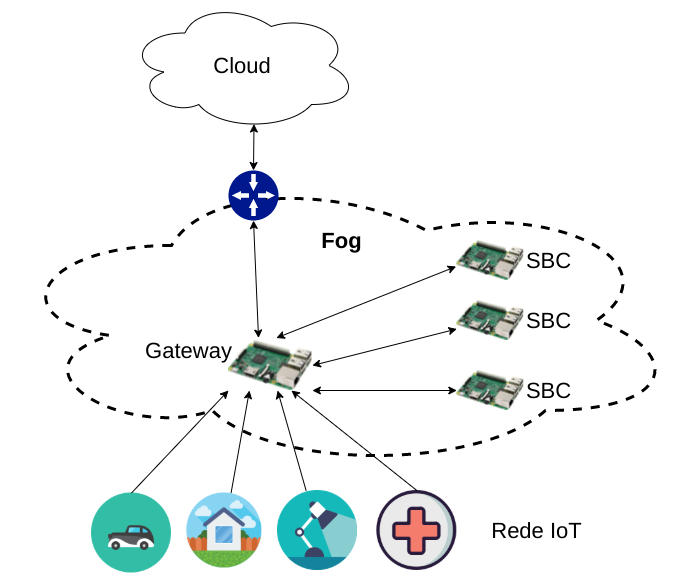
\includegraphics[width=0.8\linewidth]{figures/arq-mfog.png}
\end{frame}
\begin{frame}\centering
  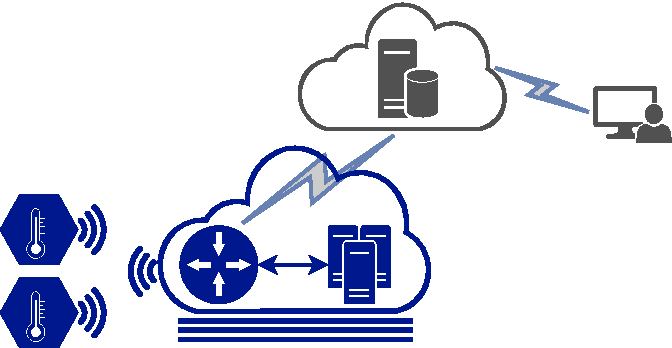
\includegraphics[width=0.8\linewidth]{figures/mfog-arch-fisica.svg.pdf}
\end{frame}
\begin{frame}\centering
  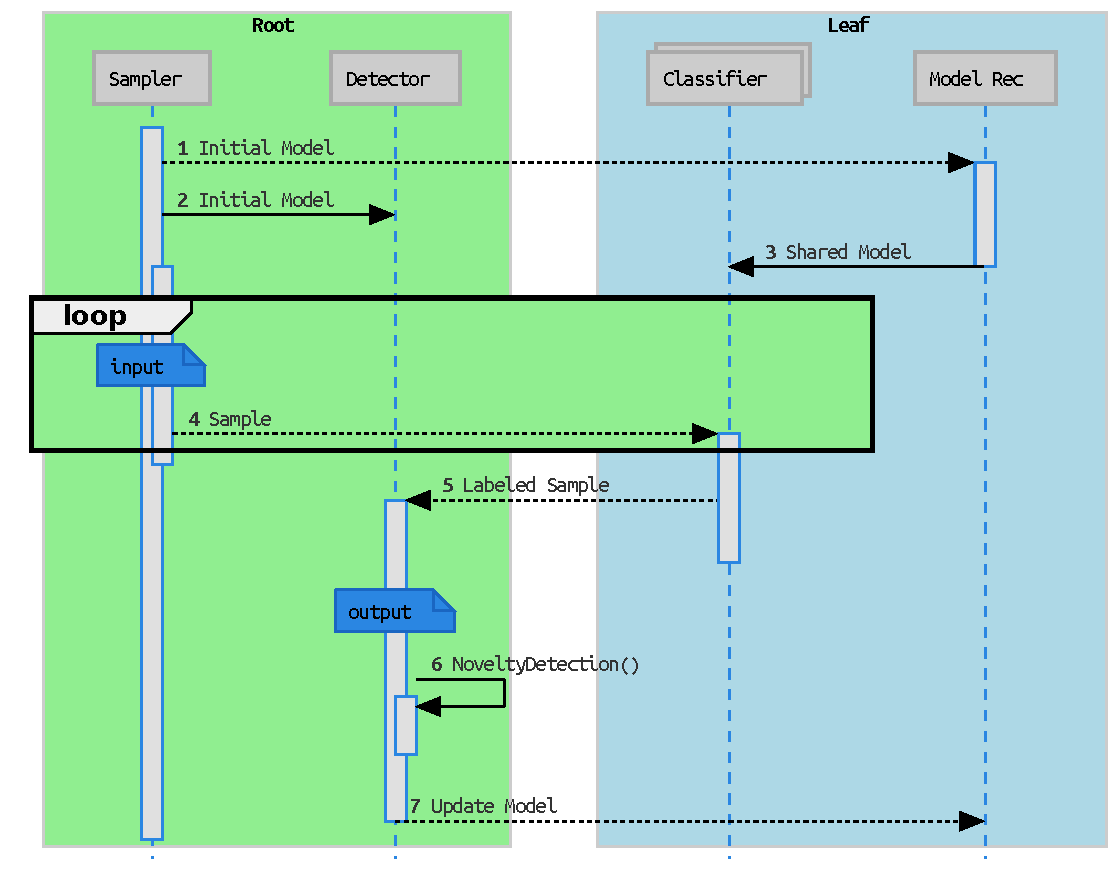
\includegraphics[width=0.93\linewidth]{figures/lifecycle-uml-svg.pdf}
\end{frame}
\begin{frame}\centering
  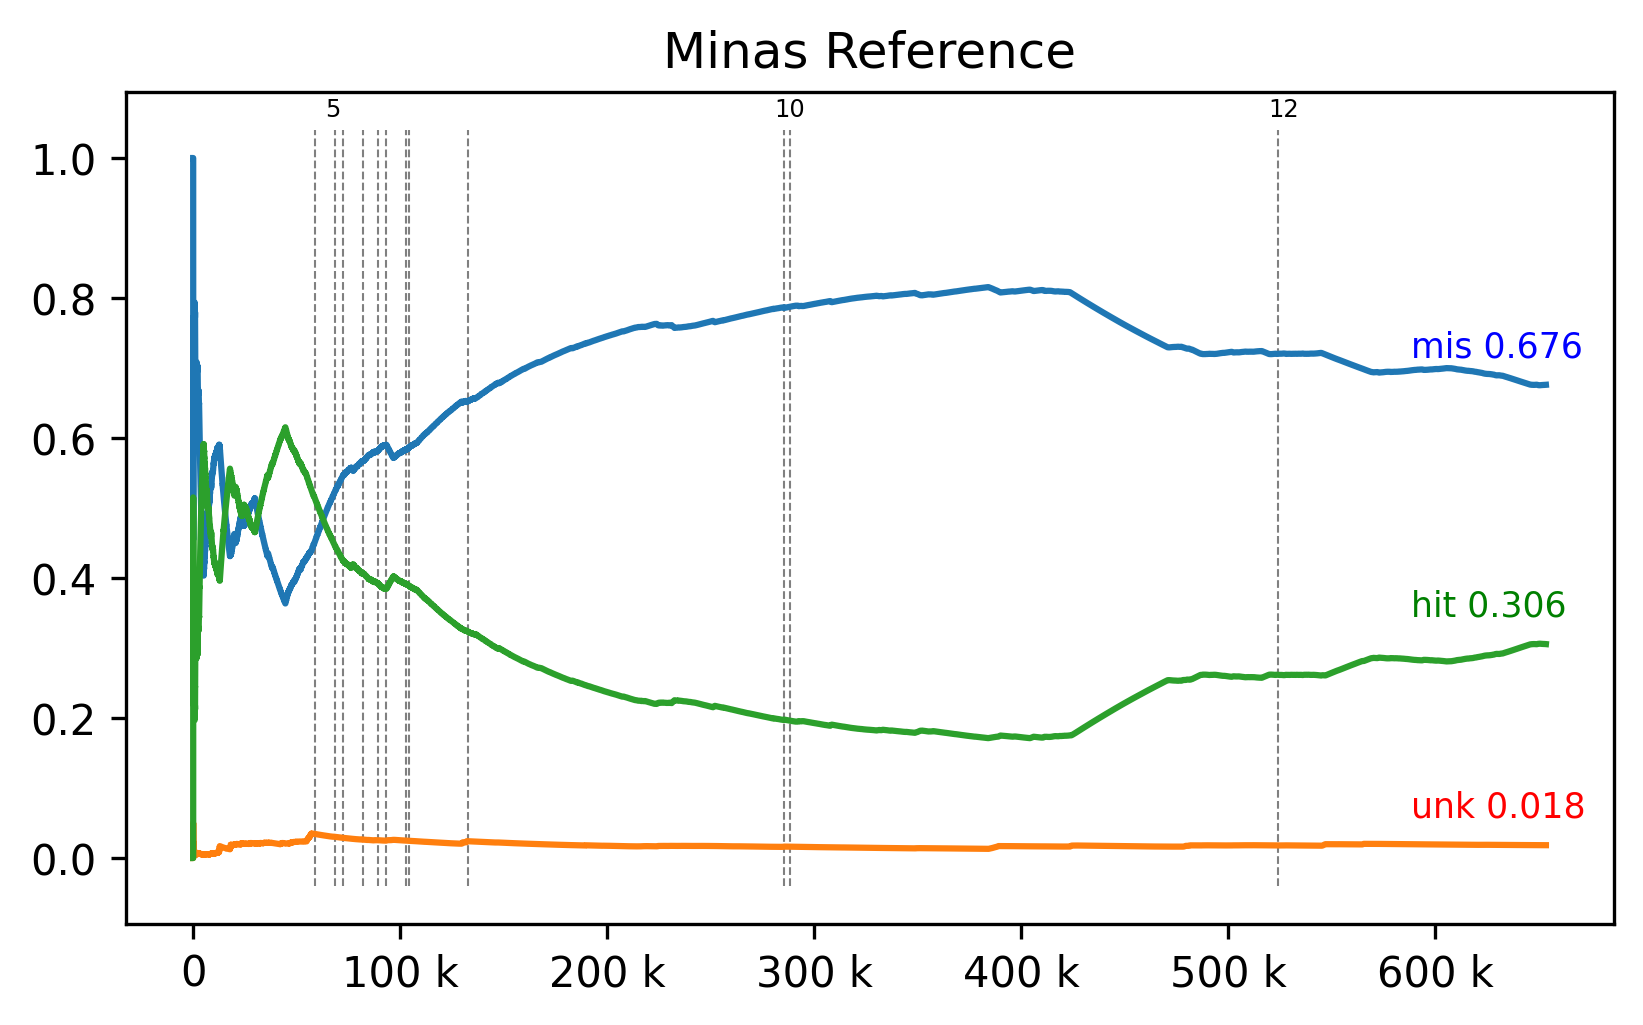
\includegraphics[width=1\linewidth]{experiments/revised-java-log.png}
\end{frame}
\begin{frame}
  % \hspace{-3cm}
  % \begin{minipage}{\paperwidth}
  \footnotesize
  \begin{table}[hbt]
    \centering
    \caption{Experimento \expA, Matriz de confusão, \emph{Kyoto} Dez. 2015.}
    \label{tab:java-matrix}
    \begin{tabular}{l *{14}{|r} }
      Rótulos   &     - &       N &    1 &    2 &    3 &  4 &   5 &    6 &    7 &     8 &    9 &    10 &   11 &  12 \\\hline
      Classes  &       &         &      &      &      &    &     &      &      &       &      &       &      &     \\\hline
      \hline
      A        &  3\;774 &  438\;750 &  123 &  145 &  368 &  8 &  52 &  165 &    1 &  1\;046 &  161 &  2\;489 &   71 &  26 \\\hline
      N        &  8\;206 &  193\;030 &    0 &   79 &   44 &  0 &   0 &    0 &  229 &   181 &  154 &  4\;066 &  289 &   0 \\\hline
      \hline
      Associação &     - &       N &    A &    A &    A &  A &   A &    A &    N &     A &    A &     N &    N &   A \\\hline
      Hits ($tp$)     &     0 &  193\;030 &  123 &  145 &  368 &  8 &  52 &  165 &  229 &  1\;046 &  161 &  4\;066 &  289 &  26 
    \end{tabular}
  \end{table}
  % \end{minipage}
\end{frame}
\begin{frame}\centering
  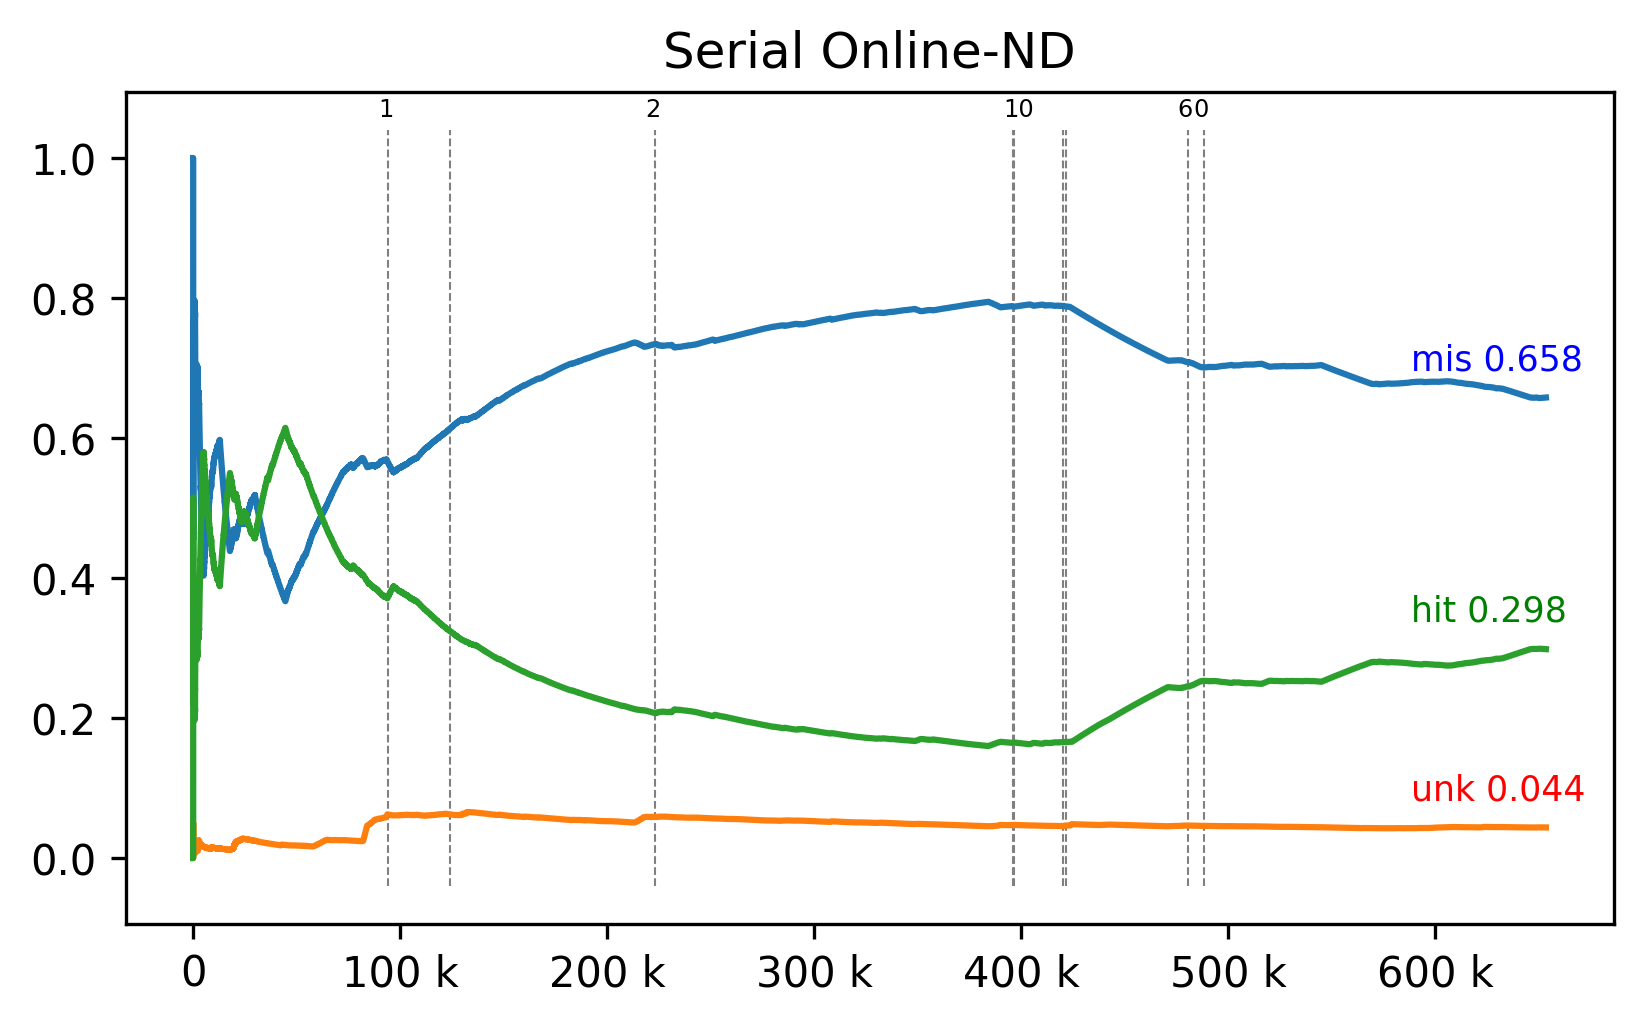
\includegraphics[width=1\linewidth]{experiments/online-nd-log.png}
\end{frame}
\begin{frame}\centering
  \begin{table}[hbt]
    \centering
    \caption{Experimento \expB, Matriz de confusão, \emph{Kyoto} Dez. 2015.}
    \label{tab:libc-matrix}
    \begin{tabular}{l|r|r|r|r|r|r|r|r|r|r|r}
      Rótulos &      - &       N &   0 &    1 &    2 &   4 &   5 &  6 &   7 &   8 &  10 \\\hline
      Classes  &        &         &     &      &      &     &     &    &     &     &     \\\hline
      \hline
      A        &  16\;086 &  429\;765 &  94 &  995 &  104 &   0 &  23 &  3 &  29 &  46 &  34 \\\hline
      N        &  12\;481 &  193\;642 &   3 &   94 &    0 &  47 &   0 &  0 &   0 &  11 &   0 \\\hline
      \hline
      Associação &      - &       N &   A &    A &    A &   N &   A &  A &   A &   A &   A \\\hline
      Hits ($tp$)     &      0 &  193\;642 &  94 &  995 &  104 &  47 &  23 &  3 &  29 &  46 &  34 
    \end{tabular}
  \end{table}
\end{frame}
\begin{frame}\centering
  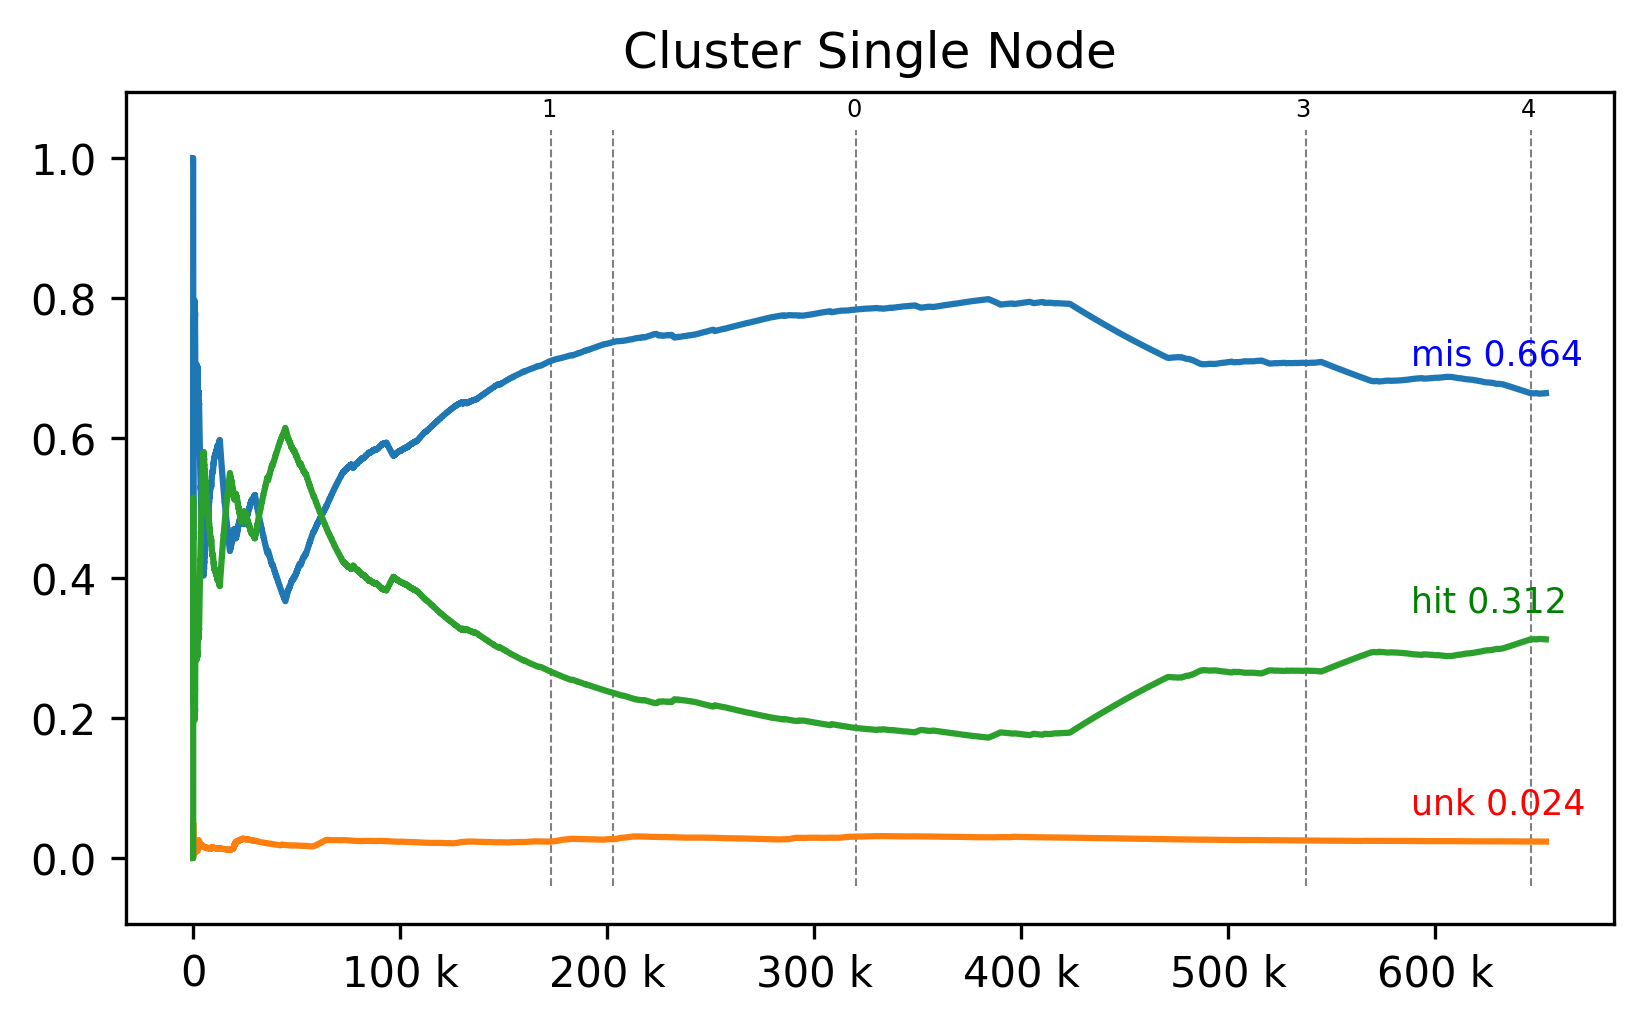
\includegraphics[width=1\linewidth]{experiments/tmi-base-log.png}
\end{frame}
\begin{frame}\centering
  \begin{table}[hbt]
    \centering
    % \setlength\tabcolsep{0.5em}
    \caption{Experimento \expC, \mfog com 1 nó e 4 núcleos, Matriz de confusão, \emph{Kyoto} Dez. 2015.}
    \label{tab:single-matrix}
    \begin{tabular}{l|r|r|r|r|r|r|r}
      Rótulos &      - &       N &    0 &    1 &   2 &  3 &  4 \\\hline
      Classes  &        &         &      &      &     &    &    \\\hline
      \hline
      A        &  12\;282 &  433\;797 &  147 &  952 &   0 &  0 &  1 \\\hline
      N        &   3\;088 &  203\;019 &   40 &   99 &  27 &  5 &  0 \\\hline
      \hline
      Associação &      - &       N &    A &    A &   N &  N &  A \\\hline
      Hits ($tp$)     &      0 &  203\;019 &  147 &  952 &  27 &  5 &  1 
    \end{tabular}
  \end{table}
\end{frame}
\begin{frame}\centering
  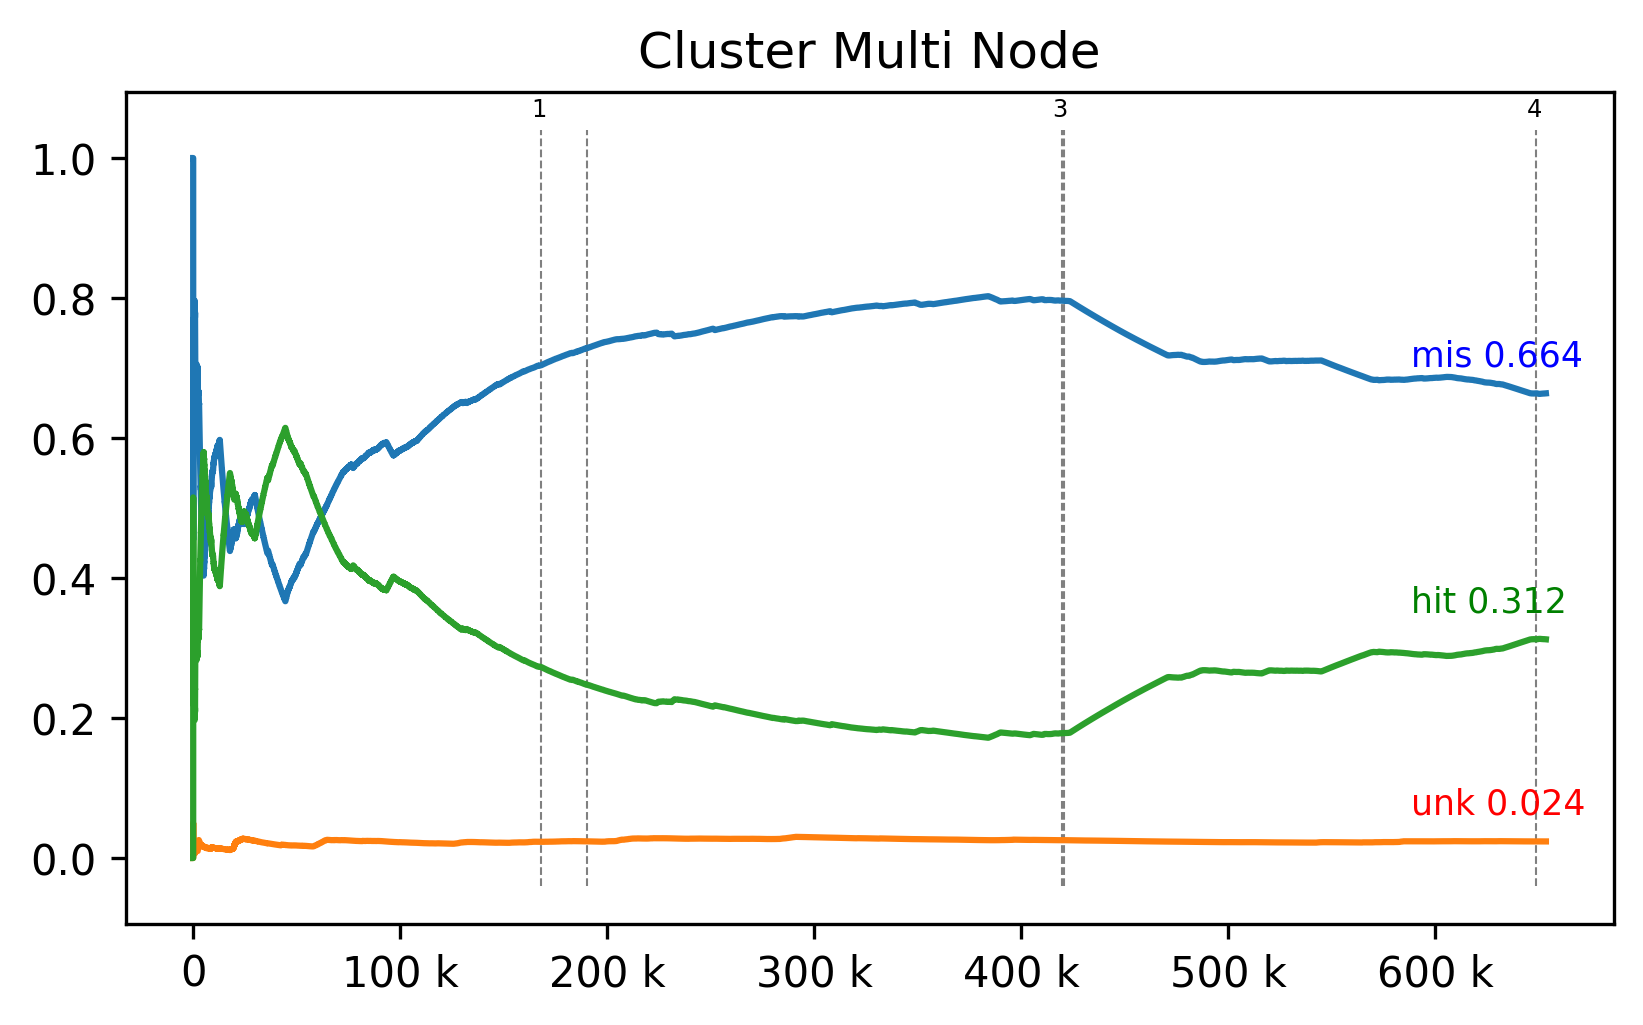
\includegraphics[width=1\linewidth]{experiments/tmi-n12-log.png}
\end{frame}
\begin{frame}\centering
  \begin{table}[hbt]
    \centering
    % \setlength\tabcolsep{0.5em}
    \caption{Experimento \expD, \mfog com 3 nós de 4 núcleos cada, Matriz de confusão, \emph{Kyoto} Dez. 2015.}
    \label{tab:multi-matrix}
    \begin{tabular}{l|r|r|r|r|r|r|r}
      Rótulos   &      - &       N &    0 &    1 &    2 &    3 &  4 \\\hline
      Classes   &        &         &      &      &      &      &    \\\hline
      \hline
      A      &  12\;378 &  433\;631 &  117 &  886 &    0 &  162 &  5 \\\hline
      N      &   3\;121 &  202\;916 &   40 &   96 &  105 &    0 &  0 \\\hline
      \hline
      Associação   &      - &       N &    A &    A &    N &    A &  A \\\hline
      Hits ($tp$)   &      0 &  202\;916 &  117 &  886 &  105 &  162 &  5 
    \end{tabular}
  \end{table}
\end{frame}
\begin{frame}\centering
  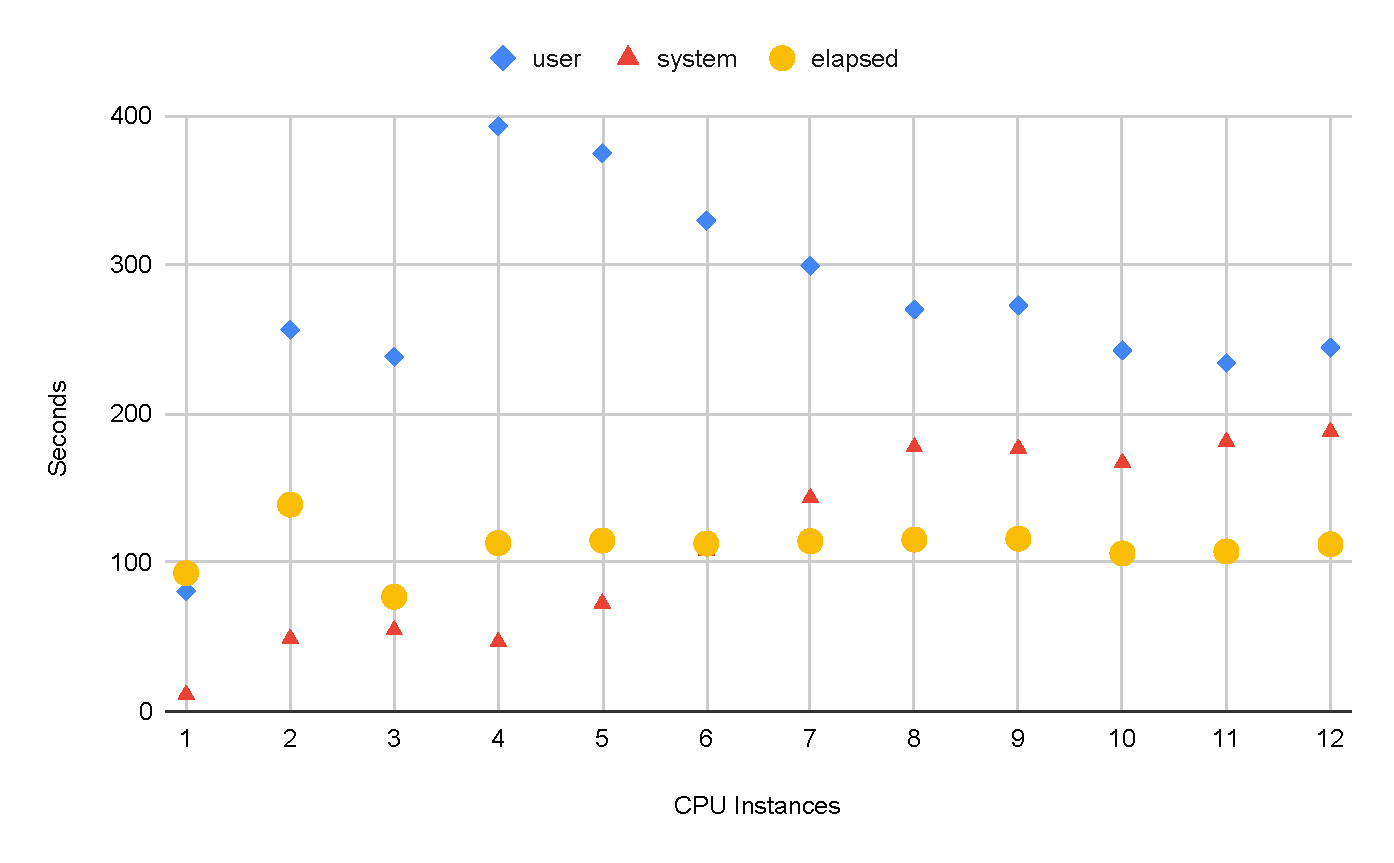
\includegraphics[width=1\linewidth,page=1]{experiments/speedup-clean.pdf}
\end{frame}
\begin{frame}\centering
  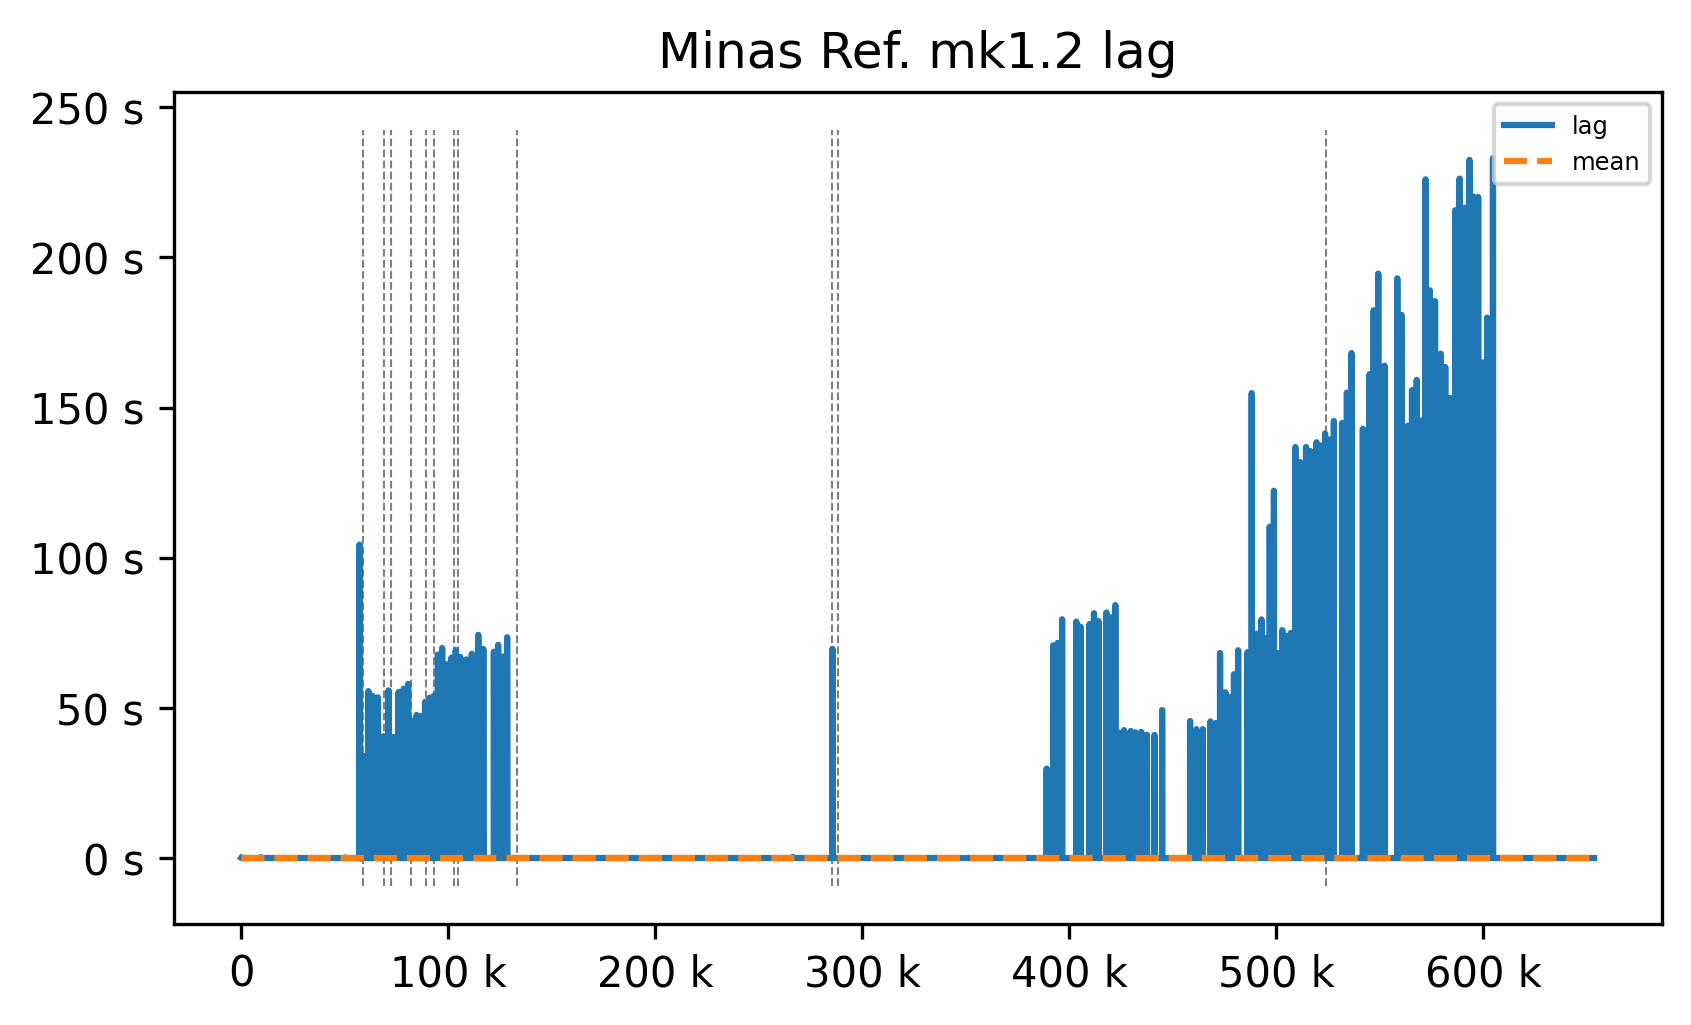
\includegraphics[width=1\linewidth]{experiments/lag-java.png}
\end{frame}
\begin{frame}\centering
  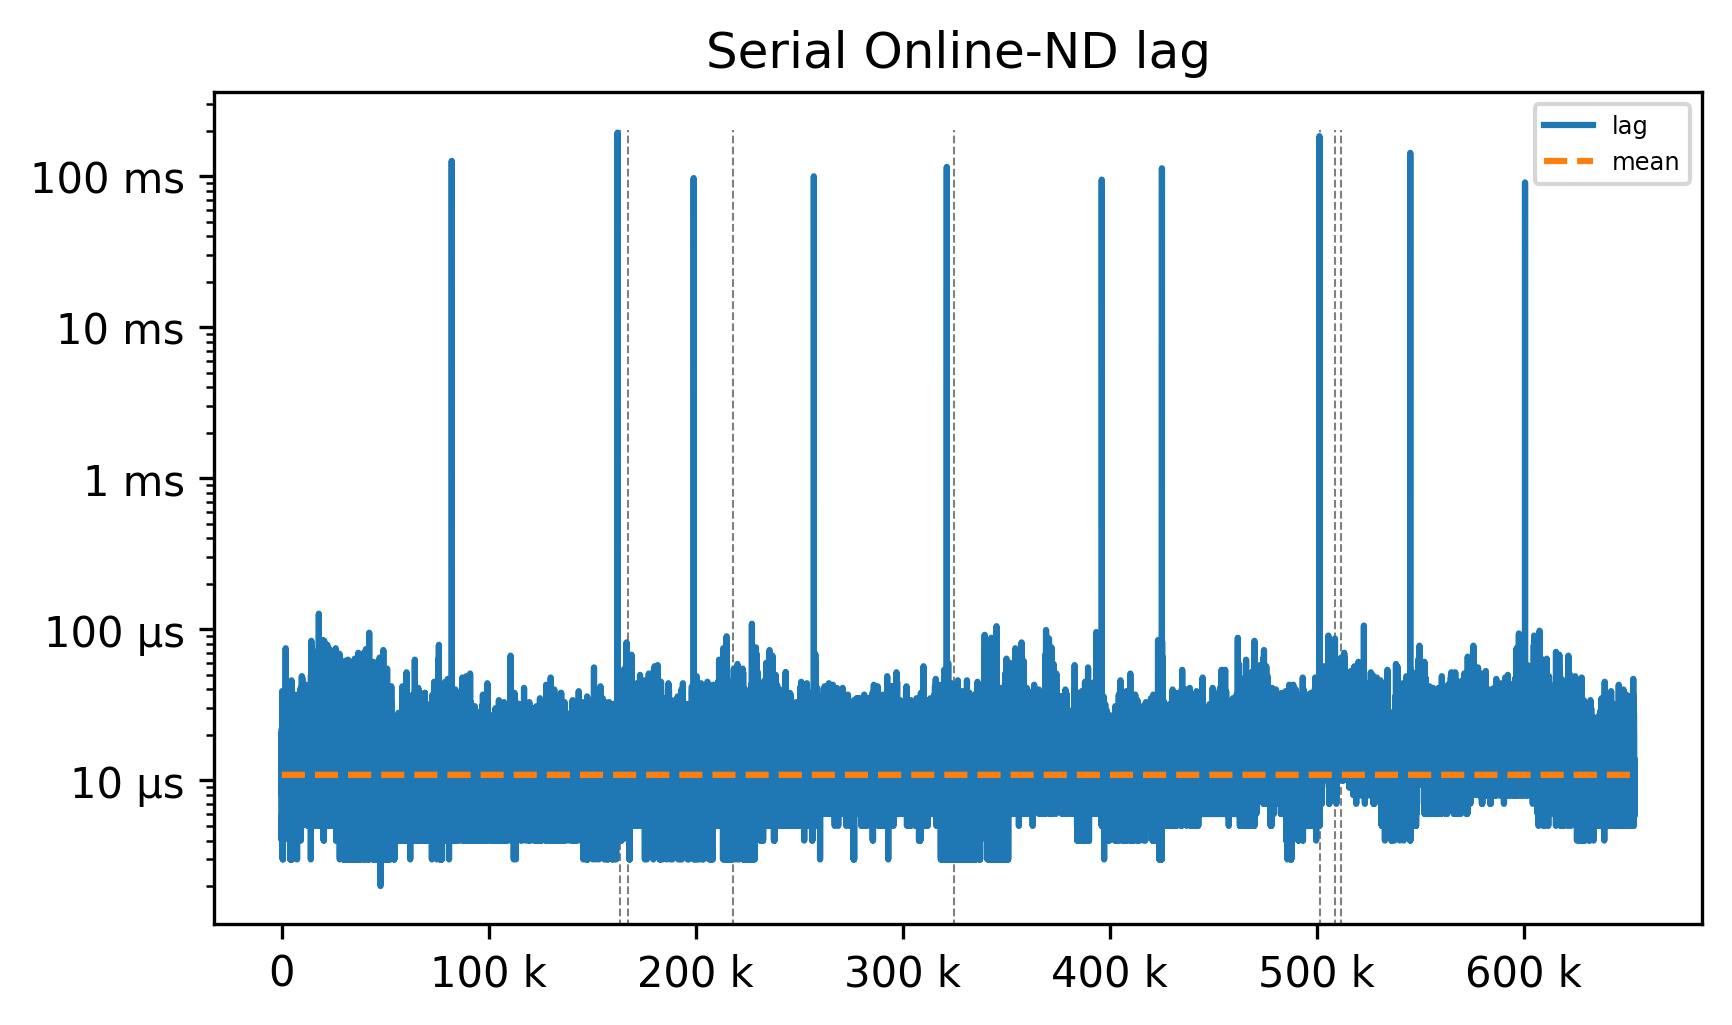
\includegraphics[width=1\linewidth]{experiments/lag-serial.png}
\end{frame}
\begin{frame}\centering
  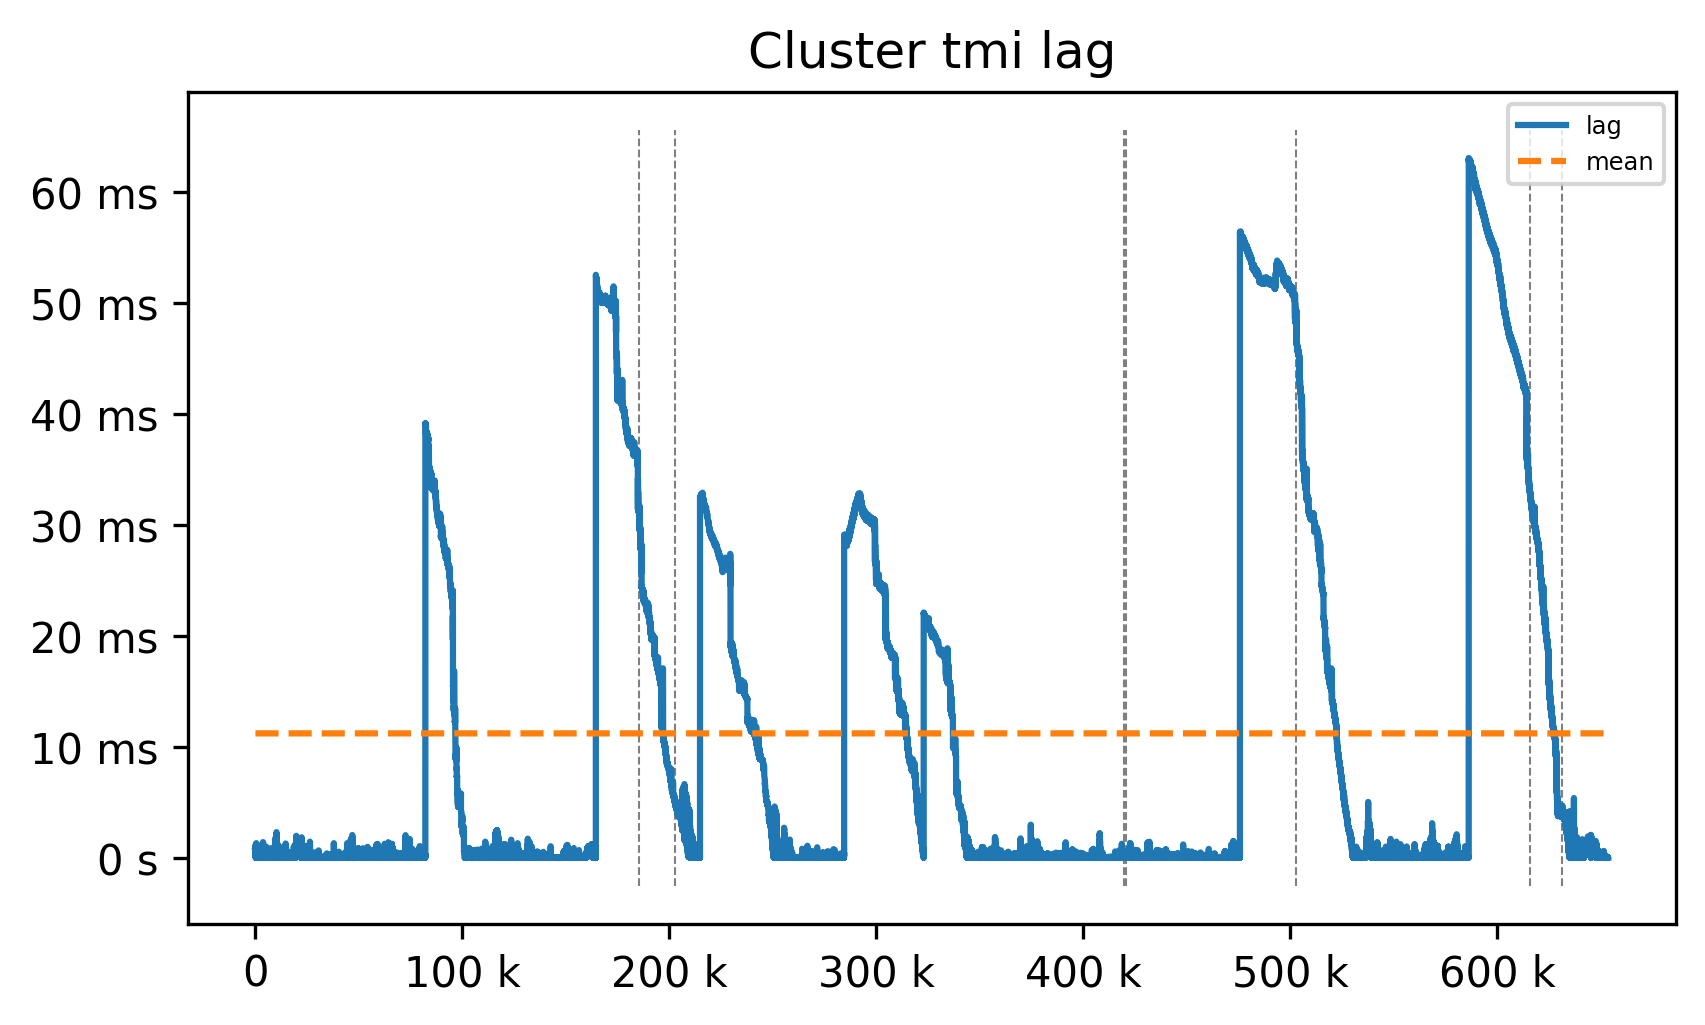
\includegraphics[width=1\linewidth]{experiments/lag-mfog.png}
\end{frame}

\end{document}
